% -----------------------------------------------
% Template for ISMIR Papers
% 2023 version, based on previous ISMIR templates

% Requirements :
% * 6+n page length maximum
% * 10MB maximum file size
% * Copyright note must appear in the bottom left corner of first page
% * Clearer statement about citing own work in anonymized submission
% (see conference website for additional details)
% -----------------------------------------------

\documentclass{article}
\usepackage[T1]{fontenc} % add special characters (e.g., umlaute)
\usepackage[utf8]{inputenc} % set utf-8 as default input encoding
\usepackage{amsmath,cite,url}
\usepackage{graphicx}

\usepackage{subcaption}

\usepackage{amssymb}
\usepackage{pifont}% http://ctan.org/pkg/pifont
\newcommand{\cmark}{\textcolor{green}{\ding{51}}}%
\newcommand{\xmark}{\textcolor{red}{\ding{55}}}%
\usepackage{multirow}
\usepackage[symbol]{footmisc}
\usepackage{booktabs}
\usepackage[table,xcdraw]{xcolor}
\usepackage{import}
\usepackage{tikz}
\usepackage{ismir} % Remove the "submission" option for camera-ready version

\newenvironment{dummyfigure}[2][htbp]
{
  \begin{figure}[#1] % Allow optional placement argument
    \centering
    \begin{tikzpicture}
      \draw[thick] (0, 0) rectangle (#2, 0.6 * #2); % Rectangle with customizable width
      \draw[thick] (0, 0.6 * #2) -- (#2, 0); % Diagonal line 1
      \draw[thick] (0, 0) -- (#2, 0.6 * #2); % Diagonal line 2
      \node at (#2 / 2, 0.3 * #2) {\textbf{Placeholder}}; % Placeholder text in center
    \end{tikzpicture}
}
{
    \end{figure}
}


\usepackage{amssymb}
\usepackage{pifont}% http://ctan.org/pkg/pifont
\usepackage{multirow}
\usepackage[symbol]{footmisc}
% \usepackage[affil-it]{authblk}
\usepackage{booktabs}
\usepackage[table,xcdraw]{xcolor}

\usepackage{tikz}
\usepackage{emoji}
\usepackage[table,xcdraw]{xcolor}
\usepackage{array}
\usepackage{graphicx}



\newcommand*\circled[1]{\tikz[baseline=(char.base)]{
            \node[shape=circle,draw,inner sep=2pt] (char) {#1};}}

\newcommand*\circledblue[1]{\tikz[baseline=(char.base)]{%
            \node[shape=circle,fill=blue!20,draw,inner sep=1pt] (char) {#1};}}

\usepackage{enumitem}

\newcommand{\redcross}{\textcolor{red}{\ding{55}}} % Red cross
\newcommand{\greencheck}{\textcolor{green}{\ding{51}}} % Green checkmark

\newcommand{\mAR}{\text{mAR}}
\newcommand{\LL}{\mathcal{L}}

\definecolor{lightgray}{RGB}{230,230,230}
\newcommand{\grayline}{\arrayrulecolor{lightgray}\hline\arrayrulecolor{black}}

\usepackage{dsfont}
% Example definitions.
% --------------------
\def\x{{\mathbf x}}
\def\L{{\cal L}}

\newcommand{\norm}[2]{\| #2 \|_{_{#1}}}

\DeclareMathOperator{\sg}{sg}

\newcommand{\alain}[1]{\textcolor{magenta}{#1}}
\newcommand{\julien}[1]{\textcolor{teal}{#1}}
\newcommand{\comm}[1]{\textcolor{red}{TODO #1}}

\usepackage{lineno}
% \linenumbers

% Title. Please use IEEE-compliant title case when specifying the title here,
% as it has implications for the copyright notice
% ------
\title{SLAP: Siamese Language-Audio Pretraining\\without negative samples for Music Understanding}

% Note: Please do NOT use \thanks or a \footnote in any of the author markup

% Single address
% To use with only one author or several with the same address
% ---------------
%\oneauthor
% {Names should be omitted for double-blind reviewing}
% {Affiliations should be omitted for double-blind reviewing}

% Two addresses
% --------------
%\twoauthors
%  {First author} {School \\ Department}
%  {Second author} {Company \\ Address}

% Three addresses
% --------------\input{ISMIR2021_paper.tex}

% Four or more addresses
% OR alternative format for large number of co-authors
% ------------
% \multauthor
% {Julien Guinot$^{1,2}$ \hspace{1cm} Elio Quinton$^2$ \hspace{1cm} George Fazekas$^1$} { 
% $^1$ School of EECS, Queen Mary University of London, London, UK\\
% $^2$ Music and Audio Machine Learning Lab, Universal Music Group, London, UK\\
% {\tt\small j.guinot, george.fazekas@qmul.ac.uk, elio.quinton@umusic.com}
%}

\multauthor
{Julien Guinot$^{*,1,2}$ \hspace{1cm} Alain Riou$^{*,3}$ \hspace{1cm} Elio Quinton$^2$ \hspace{1cm} György Fazekas$^1$} { 
$^1$ Centre for Digital Music, Queen Mary University of London, U.K.\\
$^2$ Music \& Audio Machine Learning Lab, Universal Music Group, London, U.K.\\
$^3$ LTCI, Télécom-Paris, Institut Polytechnique de Paris, France \\
{\small $^*$Equal contribution, correspondence to {\tt j.guinot@qmul.ac.uk}}
}
% For the author list in the Creative Common license, please enter author names. 
% Please abbreviate the first names of authors and add 'and' between the second to last and last authors.
%\def\authorname{Julien Guinot, Elio Quinton, George Fazekas}
% \def\authorname{Alain Riou, Julien Guinot, Elio Quinton, György Fazekas, Geoffroy Peeters}
% \def\authorname{Anonymous authors for review period}

\def\authorname{J. Guinot, A. Riou, E. Quinton, and G. Fazekas.}


% Optional: To use hyperref, uncomment the following.
\usepackage[bookmarks=false,pdfauthor={\authorname},pdfsubject={\papersubject},hidelinks]{hyperref}
% Mind the bookmarks=false option; bookmarks are incompatible with ismir.sty.

\hypersetup{
    colorlinks=true,
    linkcolor=blue,
    citecolor=blue,
    filecolor=magenta,      
    urlcolor=cyan,
    pdftitle={Overleaf Example},
    pdfpagemode=FullScreen,
    }


\sloppy % please retain sloppy command for improved formatting

\begin{document}

%
\maketitle

\begin{abstract}

%\vspace{-3pt}

Joint embedding spaces have significantly advanced music understanding and generation by linking text and audio through multimodal contrastive learning.
However, these approaches face large memory requirement limitations due to relying on large batch sizes to effectively utilize negative samples. Further, multimodal joint embedding spaces suffer from a modality gap wherein embeddings from different modalities lie in different manifolds of the embedding space.

To address these challenges, we propose Siamese Language-Audio Pretraining (SLAP), a novel multimodal pretraining framework that allows learning powerful representations without negative samples. SLAP adapts the Bootstrap Your Own Latent (BYOL) paradigm for multimodal audio-text training, promoting scalability in training multimodal embedding spaces.

We illustrate the ability of our model to learn meaningful relationships between music and text --- specifically, we show that SLAP outperforms CLAP on tasks such as text-music retrieval and zero-shot classification. We also observe competitive downstream performance on several MIR tasks, including with larger or supervised models (genre and instrument classification, auto-tagging).

Additionally, our approach has attractive properties, such as a quantifiably reduced modality gap and improved robustness to batch size variations on retrieval performance.
Finally, its novel formulation unlocks large-scale training on a single GPU through gradient accumulation. 

\end{abstract}

%\vspace{-4pt}

\section{Introduction}

%\vspace{-1pt}

Joint embedding spaces for text and audio have been foundational in recent developments in music understanding and generation.
%Multimodal contrastive learning foundation models specifically have allowed for conditioning generative models on text for controllable  music generation, and have exhibited strong representation performance on downstream tasks.
Such spaces are typically learned via Multimodal Contrastive Learning (MCL), which optimizes
%In contrastive learning, a joint embedding space between modalities is built by
a pair of encoders for maximal similarity between positive pairs, while minimizing similarity for negative pairs~\cite{clip,elizalde2023clap}.

Though widely successful, some drawbacks have been identified with this method. Recent trends for joint multimodal embedding spaces have emphasized fine-grained understanding between individual text tokens and individual timesteps of music \cite{wu2024collap, komatsu2025aligned} and need for text augmentation strategies to alleviate the lack of large scale datasets \cite{yuan2024t,manco2024augment}. A modality gap emerging from the contrastive approach has been observed, where modalities lie in separate manifolds of the embedding space \cite{Fahim2024, liang2022mind}. This leads to ``joint'' representations not being truly joint, potentially harming performance. Importantly, contrastive approaches face an inherent scalability issue. Their formulation makes them 1) dependent on batch size for representation quality and 2) more difficult to scale than masked modelling approaches due to the formulation of the contrastive loss \cite{pham2023combined}. These drawbacks pose issues for foundation models, which by usage should be scalable for adaptation on large-scale datasets. Further, text-music spaces are a many-to-many space. I.e., there is often no one single corresponding appropriate caption for a piece of music, and \textit{vice-versa}. 

% Though widely successful in both understanding and generation, some drawbacks have been identified with this method. Notably, recent work on joint multimodal embedding spaces has emphasized the need for finer alignment between individual text tokens and timesteps of music \cite{wu2024collap, komatsu2025aligned}, as well as text augmentation strategies to address the lack of large-scale datasets \cite{yuan2024t,manco2024augment}. A modality gap has also been observed in contrastive approaches, where modalities lie in separate manifolds of the embedding space \cite{Fahim2024, liang2022mind}, leading to ``joint'' representations that are not truly joint, potentially harming performance. Contrastive approaches face an inherent scalability issue: they 1) depend on batch size for representation quality and 2) are harder to scale than masked modelling approaches due to the nature of the contrastive loss \cite{pham2023combined}. These drawbacks are problematic for foundation models, which must scale to large datasets. Further, text-audio—especially text-music—spaces are many-to-many: there is often no single appropriate caption for a piece of music, and \textit{vice-versa}.



%Inspired by the scalability limitations of contrastive learning and recent work in stem retrieval towards a broader definition of compatibility in latent spaces\cite{riou2024stem},
Inspired by recent advances in Self-Supervised Learning for images and general audio~\cite{grill2020bootstrap,niizumi2021byol},
we propose \textbf{SLAP}, \textbf{S}iamese \textbf{L}anguage \textbf{A}udio \textbf{P}retraining.
We adapt Bootstrap Your Own Latent (BYOL) \cite{grill2020bootstrap} as a joint-embedding pretraining approach without negative samples to multimodal text-audio pretraining.
%We hope to alleviate
We show that SLAP alleviates both
the scalability issues
%of contrastive training approaches such as CLAP \cite{elizalde2023clap}
%, move towards a more compatibility-based joint space,
and the modality gap inherent to MCL. Our contributions are:

% Inspired by the scalability limitations of contrastive learning and recent work in stem retrieval embracing a broader definition of compatibility in latent spaces \cite{riou2024stem}, we propose \textbf{SLAP}, \textbf{S}iamese \textbf{L}anguage \textbf{A}udio \textbf{P}retraining. We adapt Bootstrap Your Own Latent (BYOL) \cite{grill2020bootstrap} as a joint-embedding pretraining approach without negative samples for multimodal text-audio pretraining. In doing so, we aim to alleviate the scalability issues of contrastive methods such as CLAP \cite{elizalde2023clap}, move towards a more compatibility-based joint space, and reduce modality gaps introduced by contrastive pretraining. Our contributions are:

%\vspace{-3pt}



\begin{enumerate}%[label=\protect\circled{\arabic*},topsep=0pt,itemsep=-1ex,partopsep=1ex,parsep=1ex]
\item We introduce a scalable, hyperparameter-robust approach to language-audio pretraining which does not require negative pairs to learn strong representations.
\item We outperform comparable contrastive models on retrieval and downstream probing.
\item We show that our approach significantly decreases the modality gap between audio and text embeddings compared to contrastive approaches.
\item Our approach enables larger batch sizes via gradient accumulation, which was previously inaccessible due to the formulation of the contrastive loss.
\end{enumerate}

%\vspace{-1pt}

To facilitate further research in this direction, we make our code available.\footnote{\hyperlink{https://github.com/Pliploop/SLAP}{https://github.com/Pliploop/SLAP}}

\section{Background}

% \subsection{Contrastive Language-Audio Pretraining}

% In contrastive learning, a model internalizes useful representations of data by learning to maximize similarity between views from the same sample or samples deemed similar through a given similarity metric \cite{}, while minimizing similarity to different samples. Multimodal contrastive learning (MCL) extends the framework of contrastive learning by comparing paired data from different modalities, and has seen extensive development and improvement in between text-image, text-video, audio-image, text-music and text-audio, and more pairwise modalities, with preliminary work on extending the framework to an arbitrary number of modalities. the first implementation of multimodal text-image contrastive learning (CLIP \cite{}) has seen widespread use for understanding tasks \cite{}, generative tasks \cite{}, and retrieval \cite{}. Further, joint text-multimodal spaces have been shown to disentangle high-level concepts, useful for interpretability and improving retrieval performance \cite{}.\\

% In the field of audio and music, multimodal contrastive learning, specifically text-audio and text-music contrastive learning, has also seen widespread adoption. Notably, CLAP \cite{} and subsequent developments building upon it \cite{} has shown high performance on audio understanding tasks \cite{} and has been largely used as a conditioning model for generative models for both audio and music \cite{}. In music-text representation learning specifically, MusCALL \cite{} and MuLan \cite{} have both shown state of the art performance on a range of downstream tasks, and have been leveraged to an extend for retrieval and generative models.

% \subsection{Developments of MCL}

% Despite the success of MCL, there are still open research directions directly addressing the observed shortcomings of Contrastive Learning for multimodal representation learning. One key issue with multimodal contrastive learning is scalability: previous studies show that contrastive learning benefits from largers batch sizes due to the presence of more negative samples for the model to learn from within a given batch. Conversely, scaling batch size for contrastive models is challenging, as the InfoNCE formulation loss precludes gradient accumulation, meaning the batch size is limited by the compute budget of a single GPU. Despite emerging work proposing workarounds to the InfoNCE loss formulation, we find there is little work directly addressing the core cause of this scalability issue, i.e. the contrastive approach. Further, MCL leads to the existence of a modality gap \cite{}, in which embeddings from different modalities lie in disjointed manifolds, which still satisfy the contrastive objective. Presumably, this gap emerges because of the initialization of the encoders for each modality as well as the lack of intra-modality constraints between projections for each modality. Previous work have attempted to reduce the modality gap, sometimes to great effect, but to our knowledge none do so by modifying the core method of multimodal representation learning.\\

% Other pregnant research directions for text-audio representation learning are 1- the improvement of fine-grained understanding between individual text tokens and audio segments and 2- the improvement of caption augmentation strategies to increase the scale of training data. The first direction has the goal of alleviating the high compression of information due to uninformed pooling in contrastive learning. In text-audio representation learning, work inspired by text-image representation learning \cite{} has mainly focused on either early fusion of modality information \cite{} or informed pooling before the contrastive objective \cite{}. The second addresses the scarcity of public training data for audio-text pairs when compared to image-text pairs through LLM augmentation for captions \cite{} or mining improved negatives and positives for existing captions \cite{}. While both directions have shown impressive improvements for text-audio joint space performance, neither address the training paradigm itself.

% \subsection{Siamese Networks}

% One notable method that has been developed to alleviate the aforementioned shortcomings of contrastive learning is Siamese Networks \cite{}, which prevent collapse not by including negative samples, but by introducing a lag between encoder parameters used to compute views of the same sample. In doing so, siamese networks prevent representation collapse by ensuring that compared representations are never exactly equal. The first implementation of siamese networks for representation learning on images was Bootstrap Your Own Latent (BYOL) \cite{}, which boasted improved performance, robustness and scalability over the contrastive simCLR approach \cite{}. BYOL was repurposed for audio representation learning in BYOL-A \cite{} with a simple augmentation chain of random cropping and mixup to produce different views. However, to the best of our knowledge, there is no method adapting siamese representation learning to multimodal representation learning, despite the desirable emergent properties that directly address issues with MCL.

%\subsection{Contrastive Language-Audio Pretraining}
\subsection{Multimodal Contrastive Learning}

%In contrastive learning, models learn representations by maximizing similarity between views of the same sample while minimizing similarity to different samples \cite{chen2020simple}.
%Multimodal contrastive learning (MCL) extends this by comparing paired data from different modalities and has been developed across various modality pairs, including
In contrastive learning, models learn representations by maximizing the similarity between two \emph{views} of an input while minimizing its similarity with \emph{negative samples}, typically by optimizing an InfoNCE loss~\cite{chen2020simple}.
While these views are typically crafted by randomly applying transforms to the input data points~\cite{chen2020simple,spijkervet2021contrastive}, Multimodal Contrastive Learning (MCL) instead relies on paired data from different modalities, such as text-image \cite{clip}, text-video~\cite{VATT}, audio-image~\cite{L3}, text-music \cite{manco2022contrastive,mulan}, and text-audio \cite{elizalde2023clap, zhu2024cacophony}.
Contrastive learning spanning more than two modalities has also been investigated~\cite{guzhov2022audioclip,girdhar2023imagebind,GRAM}.

MCL has been leveraged to great extent in multiple modalities for tasks such as understanding \cite{clip}, retrieval \cite{manco2022contrastive}, and generation \cite{ramesh2022hierarchical}, with many multimodal foundation models emerging from the approach \cite{alayrac2022flamingo,AudioFlamingo}.
% The first implementation of multimodal text-image contrastive learning, CLIP \cite{clip}, has been widely used for tasks such as understanding, generation, and retrieval. \comm{not only CLIP}
% Additionally, joint text-multimodal spaces have been shown to disentangle high-level concepts, enhancing interpretability and retrieval performance \cite{}.

MCL, specifically text-audio and text-music contrastive learning, has also been widely adopted in the field of audio and music. Notably, CLAP \cite{elizalde2023clap} and subsequent developments building upon it have demonstrated high audio understanding performance~\cite{yuan2024t,wu2024collap,zhu2024cacophony,ghosh2025reclap}.
Learned audio-text representations enable effective text-audio and audio-text retrieval by leveraging similarity metrics between modalities. Beyond catalogue navigation, these capabilities support retrieval-augmented audio captioning \cite{li2025drcap, ghosh2024recap}.
In music-text representation learning, MusCALL \cite{manco2022contrastive} and MuLan \cite{mulan} have both achieved strong performance on downstream tasks such as text-music retrieval, music classification, and zero-shot classification.
Finally, joint embedding text-audio spaces have also been leveraged to condition audio and music generative models \cite{evans2024fast,evans2024long,diffariff,liu2023audioldm,agostinelli2023musiclm}.
%\alain{Finally, audio encoders learned via contrastive learning This training strategy also enables to learn strong modality-specific encoders~\cite{Dubois2022}, and can be used as feature extractors, e.g., in multimodal LLM~\cite{AudioFlamingo,AudioFlamingo2}}
%\comm{maybe say the encoders are also used as backbone for multimodal LLM?}



%\subsection{Developments of Text-Audio MCL}\label{sec:limits}

%Improving joint text-audio embedding spaces is a vibrant research area, and current prevalent research directions include improving fine-grained understanding between individual text tokens and audio segments \cite{}, and enhancing caption augmentation strategies to increase the scale of training data \cite{}. The former aims to mitigate lossy information compression due to pooling in contrastive learning. Inspired by text-image representation learning \cite{}, recent work has focused on early fusion of modality information \cite{} or informed pooling before applying the contrastive objective \cite{}. The latter addresses the scarcity of public audio-text pair training data compared to image-text pairs by employing large language model (LLM) augmentation for captions \cite{} or mining improved negatives and positives for existing captions \cite{}. While both approaches have shown notable improvements in joint-embedding text-audio representation performances, neither addresses the core training paradigm of contrastive learining itself.

\subsection{Limitations of contrastive learning}\label{sec:limits}

% \alain{
% \begin{itemize}
%     \item Despite great success, contrastive learning suffers from a few limitations, mostly related to negative samples
%     \item common approach is to sample negatives at random, however for this to work, the distribution of the negative samples should match the data distribution~\cite{Wang2020a}, which typically requires large batch sizes to be stable
%     \item practical issue: loss has to be computed on a single GPU, which limits the maximal batch sl
%     \item workaround: SigLIP replaces the softmax in the contrastive loss by a sigmoid, which makes it computationally more practical but still requires careful and expensive communication between devices to compute the loss over the negative samples~\cite{Assran}
%     \item In addition, contrastive learning intrinsically optimizes a uniform prior for the data distribution, which has been shown detrimental for long-tailed data distributions~\cite{Assran2022}
% \end{itemize}}

% \alain{
% \begin{itemize}
%     \item In addition, latent spaces learnt via multimodal contrastive learning suffer from another issue often referred to as \emph{modality gap}: each modality's distribution does not cover the whole space but lie in a small cone, and the cones for different modalities do not overlap.
%     \item a few attempts have been proposed to reduce this gap (inter+intra modality CL, other people I forgot)
%     \item however, \cite{Fahim2024} recently found out that this modality gap is actually inherent to contrastive learning, even with a single modality, and proposes to explicitly incorporate additional loss terms to explicitly promote in-modal uniformity over the hypersphere
%     \item Overall, these limitations highlight the need of training paradigms beyond CL for multimodal representation learning
% \end{itemize}
% }

Despite its widespread success, contrastive learning faces notable limitations, typically related to its reliance on negative samples.
First, ensuring a diverse and representative set of negative samples is crucial for stable training, which usually necessitates a large batch size $B$ in practice.
However, computing the InfoNCE loss requires storing a $B \times B$ matrix of pairwise similarities on a single GPU, which limits scalability.
SigLIP \cite{SigLIP} addresses this by replacing the softmax in the criterion with a sigmoid, making distributed training more tractable, though it still demands costly inter-device communication.
In addition, contrastive learning implicitly assumes a uniform prior for the data distribution, which is detrimental in long-tailed scenarios \cite{Assran2023}.

MCL, more specifically, also suffers from an issue often referred to as the \textit{modality gap}, where embeddings from different modalities occupy non-overlapping cone manifolds in the joint latent space~\cite{liang2022mind}.
\cite{Shi2023} observe a relationship between this gap and the initial model weights and loss temperature, while recent findings suggest this problem could be intrinsic to the loss formulation itself~\cite{Fahim2024}.

% These limitations, both conceptual and practical, motivate the exploration of alternative training paradigms for multimodal representation learning.


\begin{figure*}[t]
    \centering
    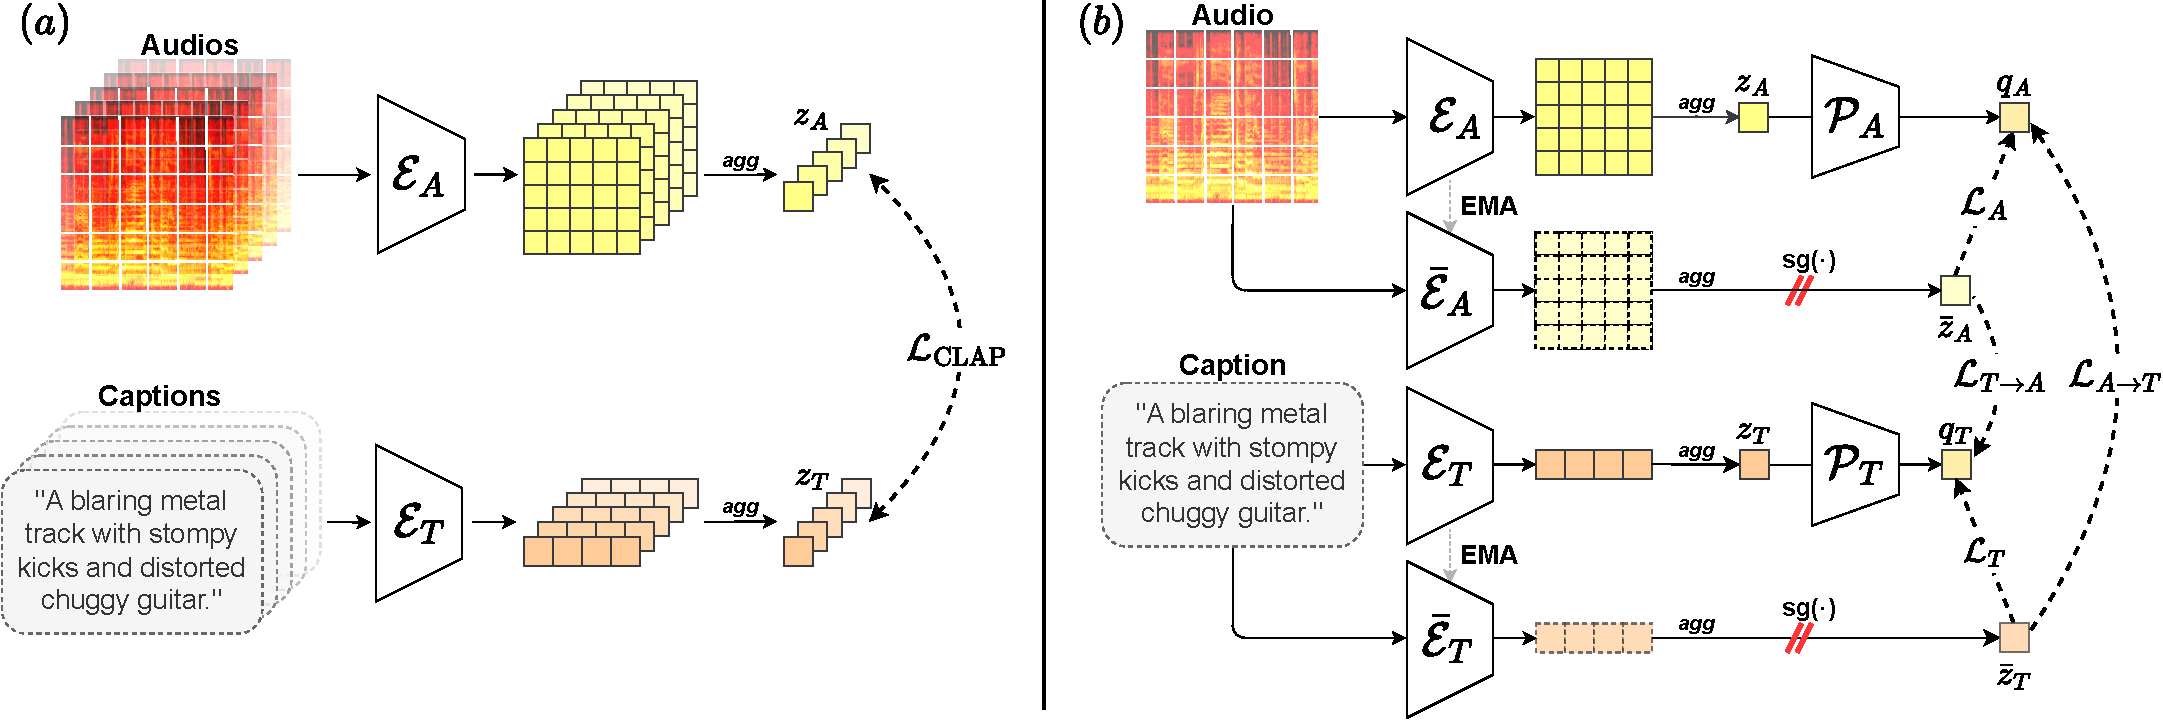
\includegraphics[width=1\textwidth]{figs/slap-ab}
    \caption{
        $(a)$ \textbf{CLAP:} The multimodal contrastive loss $\LL_{\text{CLAP}}$ is optimized between batches of audio/text pairs.
        $(b)$ \textbf{SLAP:} For each audio/text pair, we compute a query $q$ and a target $\bar{z}$ for each modality, then optimize both the intermodal losses $\LL_{A \to T}$ and $\LL_{T \to A}$ and the intramodal losses $\LL_A$ and $\LL_T$ between the queries and the targets.
        As indicated by the stop-gradient operator $\text{sg}$, the gradient flows only through the context branches, while the target encoders are updated via EMA.
        %\textbf{left} : SLAP approach - two branches, one for audio and one for text. A predictor outputs $q$ and attempts to predict the EMA-updated projection $z$ of both modalities' branches.
        %\textbf{right}: Traditional Contrastive approach (CLAP), negatives not shown.
    }
    \label{fig:model}
\end{figure*}

% Despite MCL's success, challenges remain. Scalability is a significant issue: contrastive learning benefits from larger batch sizes due to more negative samples, but the InfoNCE loss formulation limits batch size scaling and constrains it to a single GPU's compute capacity as it precludes gradient accumulation. While some workarounds have been proposed, few address the fundamental scalability issue inherent in the contrastive approach. Additionally, MCL can result in a modality gap \cite{}, where embeddings from different modalities occupy disjointed manifolds yet still satisfy the contrastive objective. Although efforts have been made to reduce this gap, they often do not modify the core multimodal representation learning method.


\subsection{Self-supervised learning without negative samples}

Recent advances in Self-Supervised Learning (SSL) have demonstrated that contrastive learning can be outperformed by alternative approaches that do not rely on negative samples, at least in unimodal settings \cite{chen2021exploring,grill2020bootstrap,assranSelfSupervisedLearningImages2023}.
%\alain{To do so, BYOL~\cite{grill2020bootstrap} leverages an asymmetric architecture composed of both a \emph{context} and \emph{target} encoders.
%Pairs of positive views, typically obtained using data augmentations, are passed through their respective encoders.
%Then a \emph{predictor} tries to predict the output of the target encoder from the one of the context.
%Importantly, the target encoder is not trained via gradient descent but its weights are updated as an Exponential Moving Average (EMA) of the ones of the context encoder.}

In particular, BYOL~\cite{grill2020bootstrap} leverages an asymmetric architecture composed of a \emph{context} encoder and a \emph{target} encoder. Two augmented views are passed through their respective encoder, and a \emph{predictor} network maps the context output to match the target's. Crucially, the target encoder is not trained via gradient descent but updated as an Exponential Moving Average (EMA) of the context encoder, which effectively avoids representation collapse~\cite{Tian2021}.

%In particular, BYOL~\cite{grill2020bootstrap} has shown that strong representations can be learned using data augmentations similar to those in SimCLR~\cite{chen2020simple}, while replacing contrastive objectives with a predictor network and a target encoder whose weights are an Exponential Moving Average (EMA) of the main one. \comm{explain BYOL mieux}


These approaches, as well as
%variants
subsequent works
relying on Transformer-based architectures, do not suffer from the conceptual limitations described in Section~\ref{sec:limits}, and achieve state-of-the-art performance in image~\cite{DINOv2,assranSelfSupervisedLearningImages2023,baevskiData2vecGeneralFramework2022} and audio~\cite{niizumi2021byol,ATST,niizumiMaskedModelingDuo2023,MATPAC} representation learning.
%A key advantage of these methods is their ability to learn richer representation spaces, as they do not suffer from the limitations inherent to CL.
However, the reliance on EMA requires the context and target encoders to share the same architecture, hindering the direct application of these methods to multimodal scenarios.

In this work, we draw inspiration from these ideas to propose a novel multimodal SSL framework that eliminates the need for negative samples while addressing the architectural limitations imposed by EMA-based methods.

% \alain{
% \begin{itemize}
%     \item unimodal case: CL has been outperformed by strategies that do not rely on negative samples
%     \item BYOL: data augmentations as in SimCLR, but predictor + EMA instead of CL
%     %\item SimSiam: EMA, while helpful is not strictly necessary. using same weights is fine
%     \item instead of data augmentations, masking (IJEPA, iBOT, data2vec)
%     \item this strategy leads to SOTA perfs in CV (DINOv2, iBOT, data2vec) and audio (BYOL-A, M2D, MATPAC)
%     \item because does not suffer from CL issues described above, can learn richer spaces
%     \item however, EMA forces to have the same architecture for both encoders, making it impractical for multimodal scenarios
%     \item in this paper, we take inspiration from these methods to propose a new multimodal SSL training strategy without negative samples
% \end{itemize}}

% \subsection{Siamese Networks}

% Siamese Networks \cite{} address some limitations of contrastive learning by preventing representation collapse without relying on negative samples; they introduce a lag between encoder parameters for computing views of the same sample, ensuring compared representations are never identical. The Bootstrap Your Own Latent (BYOL) method \cite{} applied this approach to image representation learning, demonstrating improved performance, robustness, and scalability over contrastive methods like SimCLR. BYOL was later adapted for audio representation learning in BYOL-A \cite{} using simple augmentations such as random cropping and mixup. However, to our knowledge, siamese representation learning has not yet been adapted for multimodal representation learning, despite its potential to address issues inherent in MCL.


\section{Siamese Language-Audio Pretraining}
% \begin{figure*}[t]
%     \centering
%     \begin{subfigure}[b]{0.7\textwidth}
%         \centering
%         \includegraphics[width=\textwidth]{figs/BLAP.drawio.png}
%         \caption{BLAP approach}
%         \label{fig:BLAP}
%     \end{subfigure}
%     \hfill
%     \begin{subfigure}[b]{0.54\textwidth}
%         \centering
%         \includegraphics[width=\textwidth]{figs/JEPLAP.drawio.png}
%         \caption{JEPLAP approach}
%         \label{fig:JEPLAP}
%     \end{subfigure}
%  y   \caption{Comparison of BLAP and JEPLAP approaches.}
%     \label{fig:comparison_BLAP_JEPLAP}
% \end{figure*}



%\subsection{Siamese Language-Audio Pretraining}

%Siamese Language Audio Pretraining applies a BYOL training paradigm to joint multimodal training. 
The training pipeline of SLAP is depicted in Figure~\ref{fig:model}. Consider an audio encoder $\mathcal{E}_A$ mapping samples $x_A$ of length $T_A$ from the audio space to a latent audio representation $z_a$  so that $\mathcal{E}_A : x_A \in \mathbb{R}^{T_A} \mapsto z_A \in \mathbb{R}^d$ and a text encoder mapping $N$ tokens to a tex latent space $\mathcal{E}_T : x_t \in \mathbb{N}^{N} \mapsto z_t \in \mathbb{R}^d$.

Audio and text encoders project inputs into respective modalities' latent spaces. For each modality, we
define a % implement an online
\emph{context encoder} ($\mathcal{E}$) and an Exponential Moving Average (EMA)-updated \emph{target encoder} $\Bar{\mathcal{E}}$ with EMA rate $\tau$:
\begin{equation}
    \Bar{\mathcal{E}} = \tau \Bar{\mathcal{E}} + (1-\tau) \mathcal{E}.
\end{equation}

%For the context branch of both encoders, a predictor $\mathcal{P}$ is added to make the architecture asymmetric,
For each modality, we also incorporate a \emph{predictor} $\mathcal{P}$,
which has been shown \julien{to be} necessary to prevent trivial solutions and collapse
\cite{grill2020bootstrap,Tian2021}.
The predictor of each branch processes the output $z$ of the respective context encoder and aims to predict the output $\Bar{z}$ of the target branch of both modalities.
%An Audio-to-Text predictor $\mathcal{P}_{A \longrightarrow T}$ and Text-to-Audio predictor $\mathcal{P}_{T \longrightarrow A}$ process the output of the context branch of the pair of models from each modality to predict the output of the target branch of the other modality $\bar{z}$, as well as the target projection of its own modality.
%Formally, w
We notate $q$ the output of the predictor\alain{:}
%with the context encoder projection $z$ as input and $\Bar{z}$ projections from the target encoder:

\begin{equation}
    q_A = \mathcal{P}_{A}(z_A), \qquad
    q_T = \mathcal{P}_{T}(z_T).
\end{equation}

%The loss is then computed between the EMA-encoded latent and the predicted associated latent from the other modality as the BYOL loss (i.e. normalized cosine distance between embeddings from the predictor and the projector):
The model is trained by minimizing \emph{intermodal losses}, defined as the cosine distance between the queries $q$ and targets $\bar{z}$ from different modalities:
\begin{equation}
    \mathcal{L}_{A \rightarrow T} = 1 - \frac{q_A \cdot \Bar{z}_T}{\norm{}{q_A} \norm{}{\Bar{z}_T}}, \;
    \mathcal{L}_{T \rightarrow A} = 1 - \frac{q_T \cdot \Bar{z}_A}{\norm{}{q_T} \norm{}{\Bar{z}_A}},
\end{equation}
where $\norm{}{\cdot}$ denotes the $L_2$ norm.

Additionally, we introduce \emph{intramodal losses} between the queries $q$ and targets $\bar{z}$ within each modality, which we find to empirically yield stronger retrieval performance than using intermodal losses alone (see Section \ref{subsection: role of intermodal and intramodal loss terms}):

\begin{equation}
    \mathcal{L}_{A} =  1 - \frac{q_A \cdot \Bar{z}_A}{\norm{}{q_A} \norm{}{\Bar{z}_A}}, \quad
    \mathcal{L}_{T} =  1 - \frac{q_T \cdot \Bar{z}_T}{\norm{}{q_T} \norm{}{\Bar{z}_T}}.
\end{equation}


The final loss is a combination of intramodal and intermodal losses with a weighing term $\lambda \in [0, 1]$:

\begin{equation}
    \mathcal{L} = \lambda \big(\mathcal{L}_{A \to T} + \mathcal{L}_{T \to A}\big) + (1-\lambda) \big(\mathcal{L}_{A} + \mathcal{L}_{T} \big).
\end{equation}

%Note that the gradient flows only through the context branch of each modality, as indicated by the $\text{sg}(\cdot)$ (stop-gradient) operator in Figure~\ref{fig:model}.

This approach does not require any complex machinery to prevent collapse other than an EMA update of encoders from both modalities and the addition of the symmetry-breaking predictor.

% \subsection{Joint Embedding Predictive Language Audio Pretraining}

% The previous approach alleviates the scalability issue of contrastive training, and potentially the modality gap. However, there is still no fine-grained understanding of temporal and token-wise correlations in music. We propose JEPLAP, an extension of BLAP, which extends the BYOL framework to the JEPA framework which has been well explored in image, audio, and video, but not yet in multimodal settings. Our audio and text encoders are now considered to be sequential (i.e. they do not aggregate the captions and audio chunks into a single embedding):


% \begin{equation*}
%     \mathcal{E}_T : \mathbb{N}^N \mapsto \mathbb{R}^{(N_T, d_T)}
% \end{equation*}

% \vspace{-10pt}

% \begin{equation*}
%     \mathcal{E}_A : \mathbb{R}^T \mapsto \mathbb{R}^{(N_A, d_A)}
% \end{equation*}

% In unimodal JEPA approaches and BYOL approaches, the same spatial size of the input and the output allows for symmetrical and direct predictors, taking the encoded context as input and outputting the target embedding. In our case, the ``input'' of the predictors is of shape $(N_A, d_A)$, resp. $(N_T, d_T)$, which renders a direct predictor difficult to implement. We adopt a different approach, where instead of the input to the predictor, the encoded context serves as \textbf{conditioning} for the intermodality predictor. As in other JEPA approaches, patches from the context (in both modalities) are masked and dropped out with a certain masking ratio $p$ and masking algorithm \cite{} (Discussed in section \ref{}). Figure \ref{fig:JEPLAP} shows the approach. i.e., the input to either predictor is a sequence of the same shape as the target, and the predictor leverages the information from the external modality from the conditioning (e.g. cross-attention, in-context conditioning, etc.). Considering $z_{M,A} \in \mathbb{R}^{N_A,d_A}$, $z_{M,T} \in \mathbb{R}^{N_T,d_T}$ the learned mask token for the audio and text modality copied to reach the desired sequence length, the predicted sequence is given by:

% \begin{equation*}
%     \tilde{z}_A =  \mathcal{E}(z_{M,A},\mathcal{E}(z_{T}))
% \end{equation*}

% (resp. $T,A$). The loss is computed the same as BLAP, adding the sequence length dimension. 

\section{Experimental Setup}
\subsection{Datasets} \label{subsection: Datasets}

% We train general-audio capable models on the Auto-ACD Dataset \cite{sun2024auto} which consists of 1.5 million audio-text pairs, with an average caption length of 18 words and a vocabulary of 23,000 unique words. Captions are obtained by reformatting the output of a mixture of expert image and audio captioning models on AudioSet \cite{audioset} and VGGSound \cite{chen2020vggsound} through the chatGPT API.
The list of datasets used in this work is reported in Table \ref{tab:datasets}.
We train SLAP on an internal private dataset of 260,000 pairs of full-length production-quality music tracks and professionally annotated captions (PrivateCaps \cite{manco2022contrastive}). Our retrieval testing datasets include two music-caption pair datasets. Specifically, we use MusicCaps \cite{agostinelli2023musiclm} and the Song Describer Dataset \cite{manco2023song} for text-music retrieval performance evaluation. MusicCaps contains 5,521 music clips, each accompanied by a detailed text description. The Song Describer Dataset includes 2-minute-long permissively licensed music clips with crowd-sourced single-sentence captions.

For zero-shot classification and downstream probing performance (See Sections \ref{subsection: Downstream probing}, \ref{subsection: Zero-shot performance}), we use the GTZAN dataset \cite{GTZAN} for music genre classification, which contains 1,000 audio tracks, each 30 seconds long, spanning 10 genres. We also use the MagnaTagATune (MTAT) dataset \cite{MTT}, an automatic tagging dataset consisting of 25,000 30-second music clips with 50 associated tags. Additionally, we employ the OpenMic dataset \cite{humphrey2018openmic} for fine-grained instrument tagging, containing annotations for instrument presence over 20,000 snippets.

\begin{table}%[h]
\centering
\resizebox{\columnwidth}{!}{
\begin{tabular}{llcc}
\toprule
\textbf{Task} & \textbf{Dataset} & \textbf{\# clips} & \textbf{Clip length} \\
\midrule
\multirow{1}{*}{\alain{T}raining} & PrivateCaps & 260k & full length \\
\midrule
\multirow{2}{*}{Retrieval} & MusicCaps~\cite{agostinelli2023musiclm} & 5.5k & 10 seconds \\
 & Song Describer~\cite{manco2023song} & 1k & 2 minutes \\
\midrule
\multirow{3}{*}{Probing/ZS} & GTZAN~\cite{GTZAN} & 1k & 30 seconds \\
 & MagnaTagATune~\cite{MTT} & 25k & 30 seconds \\
 & OpenMic~\cite{humphrey2018openmic} & 20k & 10 seconds \\
\bottomrule
\end{tabular}
}
\caption{Datasets used for training, retrieval, and downstream tasks (probing and zero-shot classification).}
\label{tab:datasets}
\end{table}

\begin{table*}[t]
\resizebox{\textwidth}{!}{%
\begin{tabular}{lcccccccccccccccccccccc}
\toprule
                           &            &  & \multicolumn{10}{c|}{Song Describer}                                                                                        & \multicolumn{10}{c}{MusicCaps}                                                                                            \\ \cline{4-23} 
                           &            &  & \multicolumn{5}{c|}{$A \rightarrow T$}                       & \multicolumn{5}{c|}{$T \rightarrow A$}                       & \multicolumn{5}{c|}{$A \rightarrow T$}                       & \multicolumn{5}{c}{$T \rightarrow A$}                      \\ \cmidrule{4-23} 
                           &            &  & \multicolumn{3}{c}{Recall $(\uparrow)$} & \multicolumn{2}{c|}{Norm. rank ($\downarrow$)}  & \multicolumn{3}{c}{Recall $(\uparrow)$} & \multicolumn{2}{c|}{Norm. rank ($\downarrow$)}  & \multicolumn{3}{c}{Recall $(\uparrow)$} & \multicolumn{2}{c|}{Norm. rank ($\downarrow$)}  & \multicolumn{3}{c}{Recall $(\uparrow)$} & \multicolumn{2}{c}{Norm. rank ($\downarrow$)} \\ \cmidrule{4-23} 
Model                      & Pre. &  & 1       & 5      & 10      & Med. & \multicolumn{1}{c|}{Mean} & 1       & 5      & 10      & Med. & \multicolumn{1}{c|}{Mean} & 1       & 5      & 10      & Med. & \multicolumn{1}{c|}{Mean} & 1       & 5      & 10      & Med.           & Mean          \\
\midrule


\multirow{1}{*}{SLAP} & \redcross &  & \textbf{3.3} & \textbf{13.0} & \textbf{19.7} & \textbf{5.3} &   \multicolumn{1}{c|}{\textbf{12.3}} & \textbf{3.7} & \textbf{12.5} & \textbf{19.4} & \textbf{5.4} & \multicolumn{1}{c|}{\textbf{13.8}} & \textbf{1.6} & \textbf{5.3} & \textbf{7.5} & \textbf{4.8} & \multicolumn{1}{c|}{\textbf{14.5}} & \textbf{1.2} & \textbf{4.9} & \textbf{7.9} &  \textbf{4.4} &  \textbf{13.3} \\



CLAP & \redcross &  & 3.1 & 9.6 & 14.9 & 7.3 & \multicolumn{1}{c|}{14.2}  & 2.7 & 9.7 & 15.8 & 6.7 & \multicolumn{1}{c|}{16.4} & 0.9 & 3.4 & 5.2 & 8.8 & \multicolumn{1}{c|}{18.2}  & 0.7 & 3.2 & 5.2 & 7.5 & 17.4 \\


SLAP &        \greencheck    &  & \textbf{5.7}  & \textbf{18.1} & \textbf{26.6} &\textbf{ 3.2 }& \multicolumn{1}{c|}{\textbf{8.9}} & \textbf{6.0} & \textbf{18.1}       & \textbf{ 26.4}       &   \textbf{3.6}  & \multicolumn{1}{c|}{10.5}     & \textbf{3.1} & \textbf{10.1} & \textbf{15.4} &  \textbf{1.9}   & \multicolumn{1}{c|}{\textbf{7.7}}     &      \textbf{3.0}   & \textbf{9.6} & \textbf{15.4}  & \textbf{1.9}  & 7.7 \\



CLAP &     \greencheck       &  & 5.3 & 14.9  & 22.2 &  4.3   & \multicolumn{1}{c|}{9.2} & 5.7 & 16.8 & 24.1 &  4.3   & \multicolumn{1}{c|}{\textbf{9.7}} & 2.8 & 8.3 &     10.4 &  3.0   & \multicolumn{1}{c|}{10.0}     & 2.8  & 8.7 & 14.0 & 2.2 & \textbf{7.6} \\
\midrule
\multicolumn{2}{l}{MusCALL \cite{manco2022contrastive}} &  &
1.4 & 7.0 & 14.4 & 7.8 &  \multicolumn{1}{c|}{14.7} & 1.9 & 6.8 & 12.1 & 8.8 & \multicolumn{1}{c|}{19.9} &  1.5     &  7.1   &  10.8  & 9.3  & \multicolumn{1}{c|}{17.3 }     &  0.4   &  1.6  &  3.0  & 12.8 & 21.1 \\
\multicolumn{2}{l}{CLAP$^\dagger$ \cite{wu2023large,wu2024collap}}            &  &    -     &   9.8     &       -  &   -  & \multicolumn{1}{c|}{-}     &  -       &  6.7      &   -      &   -  & \multicolumn{1}{c|}{-}     &   -      &     5.0   &   -      &  -   & \multicolumn{1}{c|}{-}     &   -      &    3.1    &    -     &       -        &       -        \\
% \multicolumn{2}{l}{\textcolor{gray}{SOTA \cite{wu2024collap}}} & & \textcolor{gray}{-}
% & \textcolor{gray}{40.5} & \textcolor{gray}{-} & \textcolor{gray}{-} & \multicolumn{1}{c|}{\textcolor{gray}{-}} 
% & \textcolor{gray}{-} & \textcolor{gray}{50.2} & \textcolor{gray}{-} & \textcolor{gray}{-} & \multicolumn{1}{c|}{\textcolor{gray}{-}} 
% & \textcolor{gray}{-} & \textcolor{gray}{10.3} & \textcolor{gray}{-} & \textcolor{gray}{-} & \multicolumn{1}{c|}{\textcolor{gray}{-}} 
% & \textcolor{gray}{-} & \textcolor{gray}{17.3} & \textcolor{gray}{-} & \textcolor{gray}{-} & \textcolor{gray}{-}
%  \\


\bottomrule
\end{tabular}%
}
\caption{
    Text-Music retrieval results. \textbf{Bolded} results indicate best results between CLAP and SLAP for either models initialized from pretrained checkpoints (\greencheck) or from scratch (\redcross). All metrics are in percentages.
    Note that results from the literature denoted by $\dagger$ are not directly comparable to ours as the training datasets differ. %Greyed out results indicate SOTA results that are not comparable due to additional architecture and/or training improvements over vanilla CLAP.
}
\label{tab:music-results}
\end{table*}

\subsection{Model architecture}

We use the same architecture as in LAION-CLAP~\cite{wu2023large}, namely HTS-AT~\cite{chen2022hts} for the audio encoder and RoBERTa~\cite{liu2019roberta} for the text encoder.
%We use the HTSAT architecture for fair comparison with CLAP \cite{elizalde2023clap} trained with contrastive learning, as our audio encoder. We employ a RoBERTA text encoder (again, for fair comparison with CLAP).
This backbone configuration leads to an overall model size of 193M parameters.

The predictor architecture is a ReLU-activated multilayer perceptron (MLP) with batch normalization. By default, we employ one 4096-wide hidden layer for the MLP. Both the prediction and projection dimensions are 512, as in CLAP \cite{elizalde2023clap}. We leave the study of predictor architecture hyperparameters as well as the influence of encoder architecture to future work.

% \subsection{Training details}

% All models are trained on the PrivateCaps dataset. We use a batch size of 768 distributed across 6 A100 GPUs, with PyTorch automatic mixed precision. Models are trained for 60 epochs. Training on PrivateCaps is adjusted for the corresponding number of steps in comparable work \cite{sun2023length} on large-scale general audio datasets. We use a linear warmup and cosine decay learning rate schedule with a maximum learning rate of $4 \times 10^{-4}$ scaled with batch size and 1/10th total epochs of warmup. We use audio augmentation in the form of specAugment \cite{park2019specaugment}, i.e. masking randomly sampled parts of the spectrogram. We empirically find this audio augmentation to lead to slight performance increases on all tasks.
% We find that, while robust to a range of values, lower EMA update rates $\tau$ lead to slightly better retrieval performance, and train models with $\tau=0.95$ by default. We leave extensive study of optimal EMA schedule and rate to follow-up work.
% We train the HTSAT and RoBERTa encoders both from scratch and initialized from pretrained checkpoints. We initialize the HTSAT backbone from a public checkpoint\footnote{\hyperlink{https://github.com/LAION-AI/CLAP?tab=readme-ov-file}{https://github.com/LAION-AI/CLAP?tab=readme-ov-file}} trained on AudioSet~\cite{audioset}, and the RoBERTA backbone from the publicly available huggingface weights\footnote{\hyperlink{https://huggingface.co/FacebookAI/roberta-base}{https://huggingface.co/FacebookAI/roberta-base}}, as in previous work \cite{sun2024auto, wu2023large}. Without compilation, training takes about 30 minutes per epoch.

\subsection{Training details}

All models are trained on PrivateCaps using a batch size of 768 across 6 A100 GPUs with PyTorch automatic mixed precision, for 60 epochs.
%Training duration is matched to comparable setups on general audio datasets \cite{sun2023length}.
We use linear warmup and cosine decay with a maximum learning rate of $4 \times 10^{-4}$ (scaled by batch size) and warmup over 1/10 of total epochs. We use SpecAugment as an audio augmentation \cite{park2019specaugment}, which improves performance slightly across tasks. We set EMA update rate $\tau = 0.95$, as we empirically find that lower values (compared to 0.996 in \cite{niizumi2021byol}) yield better retrieval performance, and leave full hyper-parameter tuning to future work. We experiment with both randomly initialized and pretrained checkpoints for HTS-AT\footnote{\hyperlink{https://github.com/LAION-AI/CLAP?tab=readme-ov-file}{https://github.com/LAION-AI/CLAP?tab=readme-ov-file}} and RoBERTa\footnote{\hyperlink{https://huggingface.co/FacebookAI/roberta-base}{https://huggingface.co/FacebookAI/roberta-base}}, and initialize the HTS-AT backbone from a public checkpoint trained on AudioSet~\cite{audioset} when initializing from pretrained.


\section{Results}

\subsection{Multimodal retrieval}

We perform Audio to Text ($A \rightarrow T$) and Text to Audio ($T \rightarrow A$) retrieval across the test datasets described in Section \ref{subsection: Datasets}. We use predictions $q$ as key and query for SLAP models (see Section \ref{Subsection:Prediction vs projection retrieval}) and projections $z$ for CLAP models. We report Recall @(1,5,10), as well as Mean and Median Normalized Rank (MNR/MdNR) \cite{SampleMatch}. We report comparable results from relevant work in literature as well as our reproduced CLAP model.
% Please add the following required packages to your document preamble:
% \usepackage{multirow}
% \usepackage{graphicx}
% Please add the following required packages to your document preamble:
% \usepackage{multirow}
% \usepackage{graphicx}
% \begin{table*}[t]
% \resizebox{\textwidth}{!}{%
% \begin{tabular}{lllcccccccccccccccccccc} \toprule
%                            &            &  & \multicolumn{10}{c|}{Clotho}                                                                                                & \multicolumn{10}{c}{AudioSet}                                                                                             \\ \cline{4-23} 
%                            &            &  & \multicolumn{5}{c|}{$A \rightarrow T$}                       & \multicolumn{5}{c|}{$T \rightarrow A$}                       & \multicolumn{5}{c|}{$A \rightarrow T$}                       & \multicolumn{5}{c}{$T \rightarrow A$}                      \\ \cline{4-23} 
%                            &            &  & \multicolumn{3}{c}{Recall $(\uparrow)$} & \multicolumn{2}{c|}{NMR ($\downarrow$)}  & \multicolumn{3}{c}{Recall $(\uparrow)$} & \multicolumn{2}{c|}{NMR ($\downarrow$)}  & \multicolumn{3}{c}{Recall $(\uparrow)$} & \multicolumn{2}{c|}{NMR ($\downarrow$)}  & \multicolumn{3}{c}{Recall $(\uparrow)$} & \multicolumn{2}{c}{NMR ($\downarrow$)} \\ \cline{1-2} \cline{4-23} 
% Model                      & Pre &  & 1       & 5      & 10      & Med & \multicolumn{1}{c|}{Mean} & 1       & 5      & 10      & Med & \multicolumn{1}{c|}{Mean} & 1       & 5      & 10      & Med & \multicolumn{1}{c|}{Mean} & 1       & 5      & 10      & Med           & Mean          \\ \cline{1-2} \cline{4-23} 
% \multirow{2}{*}{AudioSLAP} &  \redcross          &  &         &        &         &     & \multicolumn{1}{c|}{}     &         &        &         &     & \multicolumn{1}{c|}{}     &         &        &         &     & \multicolumn{1}{c|}{}     &         &        &         &               &               \\
%                            &     \greencheck       &  &         &        &         &     & \multicolumn{1}{c|}{}     &        &        &         &     & \multicolumn{1}{c|}{}     &         &        &         &     & \multicolumn{1}{c|}{}     &         &        &         &               &               \\
% \multirow{2}{*}{AudioCLAP} &     \redcross       &  &         &        &         &     & \multicolumn{1}{c|}{}     &         &        &         &     & \multicolumn{1}{c|}{}     &         &        &         &     & \multicolumn{1}{c|}{}     &         &        &         &               &               \\
%                            &     \greencheck       &  &         &        &         &     & \multicolumn{1}{c|}{}     &         &        &         &     & \multicolumn{1}{c|}{}     &         &        &         &     & \multicolumn{1}{c|}{}     &         &        &         &               &               \\ \hline
%                            \multirow{1}{*}{CLAP \cite{}}      &         &  &         &        &         &     & \multicolumn{1}{c|}{}     &         &        &         &     & \multicolumn{1}{c|}{}     &         &        &         &     & \multicolumn{1}{c|}{}     &         &        &         &               &               \\
% \multirow{1}{*}{CLAP \cite{}}      &         &  &         &        &         &     & \multicolumn{1}{c|}{}     &         &        &         &     & \multicolumn{1}{c|}{}     &         &        &         &     & \multicolumn{1}{c|}{}     &         &        &         &               &               \\ \bottomrule
                           
% \end{tabular}%
% }
% \caption{General Text-Audio Retrieval results}
% \label{tab:audio-results}
% \end{table*}



We report retrieval results in Table \ref{tab:music-results}. We find that SLAP consistently outperforms both CLAP, as reported in the literature, and our own reproduced CLAP models. Notably, Recall and Normalized Rank are improved across all metrics except for the $T \rightarrow A$ task on MNR. Initializing from pretrained encoders leads to significantly better performance both for CLAP and SLAP.% It is noteworthy that our approach achieves competitive results without extra architectural tweaks or costly data augmentation as in \cite{wu2024collap,manco2024augment,yuan2024t, zhu2024cacophony}.

\begin{table}[h]
\centering
\resizebox{\columnwidth}{!}{%
\begin{tabular}{lcccc|cccc}
\toprule
& \multicolumn{4}{c}{Song Describer} & \multicolumn{4}{c}{MusicCaps} \\
\cmidrule{2-9} 
 & \multicolumn{2}{c}{$A \rightarrow T$} & \multicolumn{2}{c}{$T \rightarrow A$} & \multicolumn{2}{c}{$A \rightarrow T$} & \multicolumn{2}{c}{$T \rightarrow A$} \\
\midrule
Anchor & R@5 & MdNR & R@5 & MdNR & R@5 & MdNR & R@5 & MdNR \\ \midrule
$z$ & 17.8 & 3.6 & 17.0 & 3.8 & 9.6 & 2.1 & 9.4 & 2.3 \\
$q$ & \textbf{18.1} & \textbf{3.2} & \textbf{18.1} & \textbf{3.6} & \textbf{10.1} & \textbf{1.9} & \textbf{9.6} & \textbf{1.9} \\
\bottomrule
\end{tabular}%
}
\caption{Retrieval results using predictions $q$ or projection embeddings $z$ as anchors. Best results are in \textbf{bold}.}
\label{Projection-Prediction}
\end{table}

\subsubsection{Prediction vs. projection retrieval}\label{Subsection:Prediction vs projection retrieval}

One variant of our approach is to use predictions instead of projections to perform retrieval. Given the loss formulation, both are possible since both exist in separate embedding spaces and the pretraining objective optimizes for four-way similarity. Here we observe the effect of using $q$ or $z$ as query and key for retrieval. Results are reported in Table \ref{Projection-Prediction}. We find that using projections instead of predictions leads to a small drop in performance, but both are viable for retrieval tasks, meaning there is no loss of information when compared to CLAP for projections.

\input{tables/probing}

\subsection{Downstream probing} \label{subsection: Downstream probing}

This section verifies the quality of the learned representations of SLAP by performing downstream probing on a range of tasks on representations \textit{before} the projection head which outputs $z$. For downstream task evaluation, we freeze the audio encoder and train shallow nonlinear probes (one ReLU-activated 512-wide hidden layer MLPs). Probes are trained with a learning rate of $10^{-4}$ with an early-stopping mechanism on validation loss.

Our results are reported in Table~\ref{tab:probingtable}. As above, we compare them to our CLAP baseline and MusCALL. We report the performance of  MATPAC~\cite{MATPAC}, the current self-supervised state-of-the-art on these tasks as well.
As a reference, we also indicate state-of-the-art performances for each task.

% We compare to CLAP-extracted representations.
% Results are reported Table \ref{tab:probingtable}. We also report results from the MARBLE benchmark and results from relevant literature with text-music joint embedding training.

We observe that SLAP consistently outperforms CLAP and MusCALL, demonstrating the advantages of our target encoder/predictor strategy over contrastive learning.
%It also significantly outperforms Jukebox on all tasks.

On MTAT and OpenMic, SLAP surpasses MATPAC, which also employs a target encoder and predictor but is trained on audio alone. This suggests that language supervision is particularly beneficial for tagging tasks but is less useful for genre classification (82.9\% vs. 85.9\%).

On tagging tasks, SLAP achieves state-of-the-art results on MTAT (45.8\% vs. 41.1\%) and bridges the gap with best supervised methods on OpenMic (86.2\% vs. 86.7\%).

% - SLAP consistently outperforms CLAP, MusCALL : EMA better than CL
% - also outperforms JukeBox
% - on MTAT and OpenMic, we also outperform MATPAC, which also relies on a target encoder and a predictor but is trained on audio only.
% - this indicates that language supervision is particularly beneficial for tagging tasks (MTAT and OpenMic), but less useful for genre classification (82.9\% accuracy vs 85.9\% for MATPAC).
% - in terms of mean Average Precision, we outperform SOTA methods on on MTAT (45.8\% vs 41.1\%) and bridge the gap with supervised SOTA on OpenMic (86.2\% vs 86.7\%).

% We find that SLAP surpasses CLAP once again on all metrics for the evaluation tasks, for the same evaluation parameters. Notably, SLAP approaches state-of-the-art performance on OpenMic and MTAT, despite not being specifically fine-tuned on these datasets. 

\subsection{Zero-shot performance} \label{subsection: Zero-shot performance}

Similar to shallow downstream probing, we evaluate the zero-shot performance of SLAP by retrieving the highest similarity prompts to audio using prompts as a class proxy on GTZAN, MTAT, and OpenMic. We report Zero-shot accuracy on GTZAN, as well as ROC-AUC and mAP for automatic tagging on MTAT, and mAR on OpenMic. As previous work has shown the importance of prompt engineering for zero-shot performance \cite{manco2022contrastive}, we evaluate across four prompts with which we wrap the target class ``\{\}'', ``\{\} music'', ``this sounds like \{\}'', and ``A \{\} track''.
We report the best of four scores across datasets for both CLAP, SLAP, and MusCALL~\cite{manco2022contrastive}.

We adapt another metric for zero-shot evaluation of multilabel approaches, which we call mean Average Recall (mAR). Previous approaches evaluate multi-tag zero-shot performance by using tag-wise cosine similarity as logits as input for standard metrics such as AUROC and mAP. These metrics are not robust to to cosine similarity distributions centered around 0.5 with low spreads for certain tasks, e.g. instrumentation.
% Previous methods using cosine similarities between prompt and audio as logits for AUROC and mAP evaluation \cite{manco2022contrastive} are less robust due to
% the similarity distribution being centered around 0.5 for some tasks (e.g., instrumentation). \comm{c pas clair}
mAR computes the mean rank of retrieved ground truth tags for a given audio:% $\mAR = \frac{1}{NK} \sum_{k=0}^K{\sum}_{n=0}^N R_n@k$, 
\begin{equation}
    \mAR = \frac{1}{NK} \sum_{k=0}^K \sum_{n=0}^N R_n@k.
\end{equation}
where $K$ is the number of samples in the dataset, $N$ the number of tags, and $R_n@k$ recall at $k$ for tag $n$. We evaluate mAR on OpenMic. Results are reported in Table \ref{tab:zero} for CLAP, SLAP, and MusCALL \cite{manco2022contrastive}.

We observe that SLAP consistently outperforms or is on par with our CLAP baseline and MusCALL.
As for retrieval, a plausible cause is the better overlap between the audio and text spaces of our approach compared to contrastive ones. We measure this overlap in Section~\ref{modalitygap}.

%SLAP surpasses CLAP on all metrics but MTAT AUROC, presumably due to the high variation of the metric due to prompt compatibility observed in previous work \cite{manco2022contrastive}, and the previously mentioned distribution of similarities. With the exception of this metric, SLAP outperforms both our re-implementation of CLAP and MusCALL \cite{manco2022contrastive}.

% Please add the following required packages to your document preamble:
% \usepackage{graphicx}
% Please add the following required packages to your document preamble:
% \usepackage{multirow}
% \usepackage{graphicx}
% \begin{table}[h]
% \resizebox{\columnwidth}{!}{%
% \begin{tabular}{lllllll}
% \hline
% Model  & Prompt                  &  & \multicolumn{1}{c}{GTZAN} & \multicolumn{2}{c}{MTAT} & \multicolumn{1}{c}{OpenMIC} \\ \cline{4-7}
%        &                         &  & \multicolumn{1}{c}{Acc.}  & \multicolumn{1}{c}{AUROC} & \multicolumn{1}{c}{AP} & \multicolumn{1}{c}{Acc.} \\ \hline
% \multirow{3}{*}{SLAP} 
%        & \{\}                    &  &                           &                           &                          &                           \\
%        & \{\} music              &  &                           &                           &                          &                           \\ 
%        & one can hear \{\} here  &  &                           &                           &                          &                           \\ \hline
% \multirow{3}{*}{CLAP} 
%        & \{\}                    &  &    47.5                   &             75.3          &                 25.9     &                           \\
%        & \{\} music              &  &    39.3                       &             76.0              &     25.0                    &                           \\ 
%        & This sounds like \{\}  &  &    51.7                       &  75.9                         &            25.0              &                           \\ \bottomrule
% \end{tabular}%
% }
% \caption{Zero-shot classification and tagging results for genre and instrument classification, and automatic tagging}
% \label{tab:my-table}
% % \end{table}
% \begin{table}[h]
% \resizebox{\columnwidth}{!}{%
% \begin{tabular}{lllcccc}
% \hline
% Model  & Prompt                  &  & \multicolumn{1}{c}{GTZAN} & \multicolumn{2}{c}{MTT} & \multicolumn{1}{c}{OpenMIC} \\ \cline{4-7}
%        &                         &  & \multicolumn{1}{c}{Acc.}  & \multicolumn{1}{c}{AUROC} & \multicolumn{1}{c}{mAP} & \multicolumn{1}{c}{mAR} \\ \hline
% \multirow{5}{*}{SLAP} 
%        & \{\}                    &  & 53.7 & 75.0 & 25.7 & 70.5 \\
%        & \{\} music              &  & 54.9 & 74.4 & 27.5 & 69.0 \\ 
%        & This sounds like \{\}   &  & 58.3 & 74.5 & 31.5 & 68.8 \\ 
%        & A \{\} Track            &  & 52.7 & 72.6 & 26.7 & 69.5 \\ \cline{2-7}
%        & Average                 &  & \textbf{54.9 $\pm 2.0$}   & 74.0 $\pm0.3$   &  \textbf{27.9} $\pm 0.2$  & \textbf{69.5}$\pm0.6$ \\ \hline
% \multirow{5}{*}{CLAP} 
%        & \{\}                    &  & 47.2 & 74.3 & 25.9 & 69.8 \\
%        & \{\} music              &  & 50.2 & 75.0 & 25.0 & 68.4 \\ 
%        & This sounds like \{\}   &  & 51.7 & 74.8 & 26.0 & 68.8 \\ 
%        & A \{\} Track            &  & 47.2 & 72.7 & 23.9 & 70.1 \\ \cline{2-7}
%        & Average                 &  & 46.7 $\pm 4.1 $ & \textbf{74.2} $\pm 0.8$ & 25.2 $\pm 0.8$ & 69.3 $\pm0.5$ \\ \hline  
% \multirow{1}{*}{MusCALL} 
%        & Average                 &  & 47.6$\pm0.6$   &   73.6$\pm0.2$ & 22.8$\pm0.2$   & 66.3$\pm0.4$ \\ \midrule
       
% % \multirow{1}{*}{Lit. \cite{}} 
% %        & Average                 &  & 47.6$\pm0.6$   &   73.6$\pm0.2$ & 22.8$\pm0.2$   & 66.3$\pm0.4$ \\ \bottomrule
% \end{tabular}%
% }
% \caption{Zero-shot classification and tagging results for genre and instrument classification, and automatic tagging}
% \label{tab:zero}
% \end{table}

\begin{table}[h]
\centering
\resizebox{\columnwidth}{!}{%
\begin{tabular}{lcccccc}
\toprule
 & \multicolumn{1}{c}{GTZAN} &  & \multicolumn{2}{c}{MTAT} &  & \multicolumn{1}{c}{OpenMIC} \\
\cmidrule{2-2} \cmidrule{4-5} \cmidrule{7-7}
Model & \multicolumn{1}{c}{Acc.} &  & \multicolumn{1}{c}{AUROC} & \multicolumn{1}{c}{mAP} &  &\multicolumn{1}{c}{mAR} \\
\midrule
SLAP   & \textbf{58.3} &  & \textbf{75.0} & \textbf{31.5} &  & \textbf{70.5} \\
CLAP   & 51.7 &  & \textbf{75.0} & 26.0 &  & 70.1 \\
\midrule
MusCALL \cite{manco2022contrastive} &
48.2 &  & 73.8 & 23.0 &  & 66.7 \\
\bottomrule
\end{tabular}%
}
\caption{Best-of-four zero-shot classification and tagging results for genre and instrument classification, and automatic tagging. Best scores are shown in \textbf{bold}.} 
\label{tab:zero}
\end{table}

\begin{figure}[t]
    \centering
    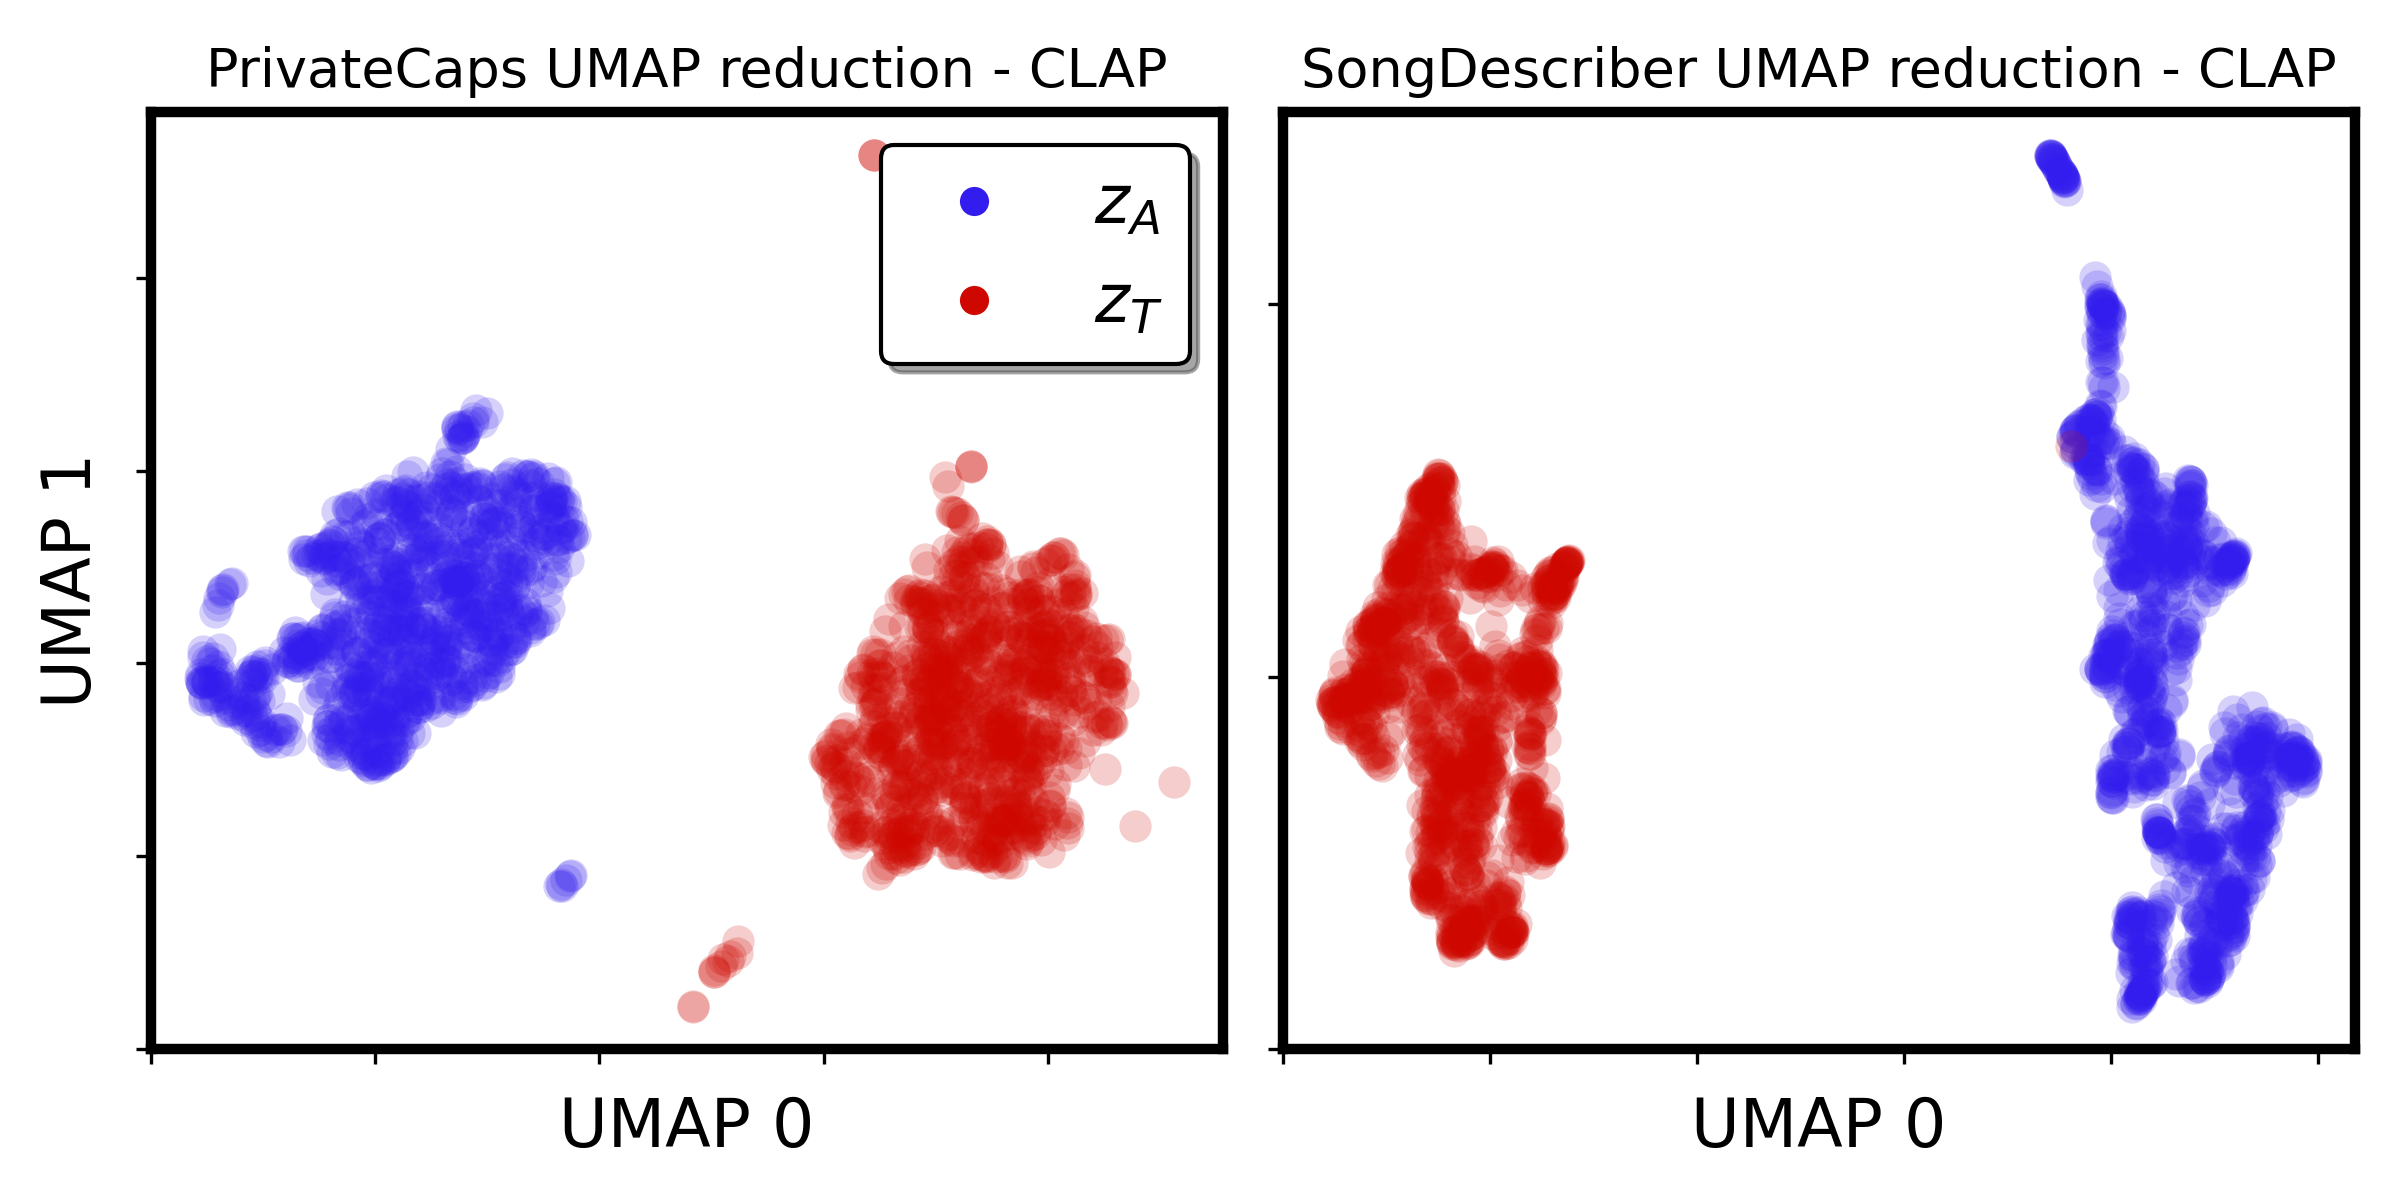
\includegraphics[width=\linewidth]{figs/umapclap.png}
    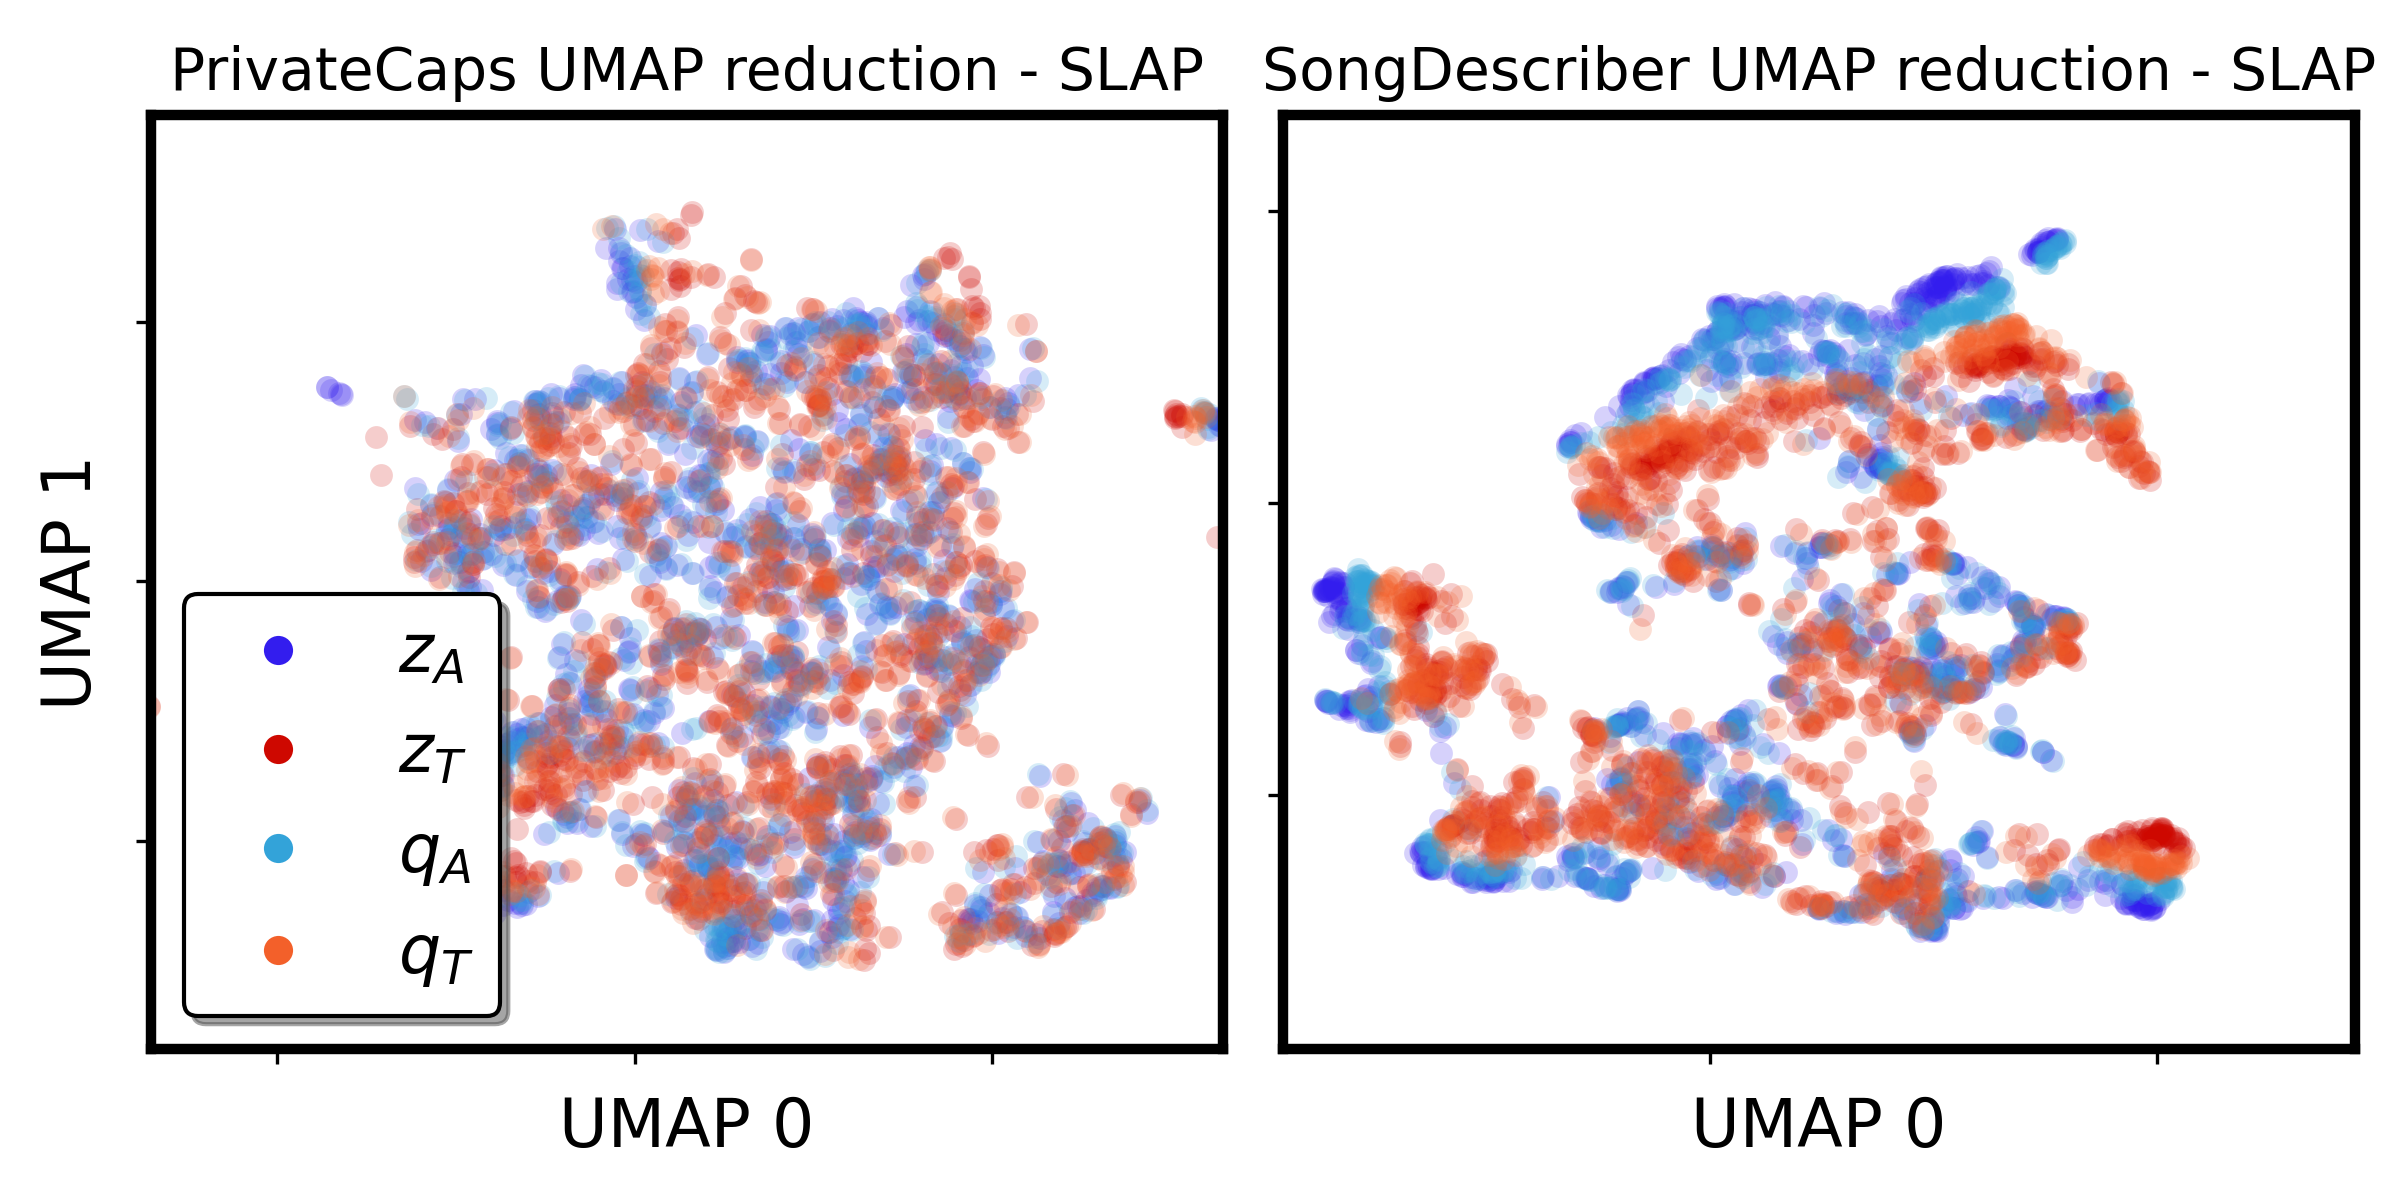
\includegraphics[width=\linewidth]{figs/umapslap.png}
    \caption{
        %UMAP Reduction of PrivateCaps (PC) and Song Describer (SD) for CLAP (\textbf{top)} and SLAP \textbf{(bottom)}.
        UMAP reduction of the CLAP (\textbf{top}) and SLAP (\textbf{bottom}) embeddings obtained from the test sets of PrivateCaps (\textbf{left}) and Song Describer (\textbf{right}).
    }
    \label{fig:UMAPreductions}
\end{figure}

% \begin{figure}[t]
%     \centering
%     \begin{subfigure}{\columnwidth}
%         \centering
%         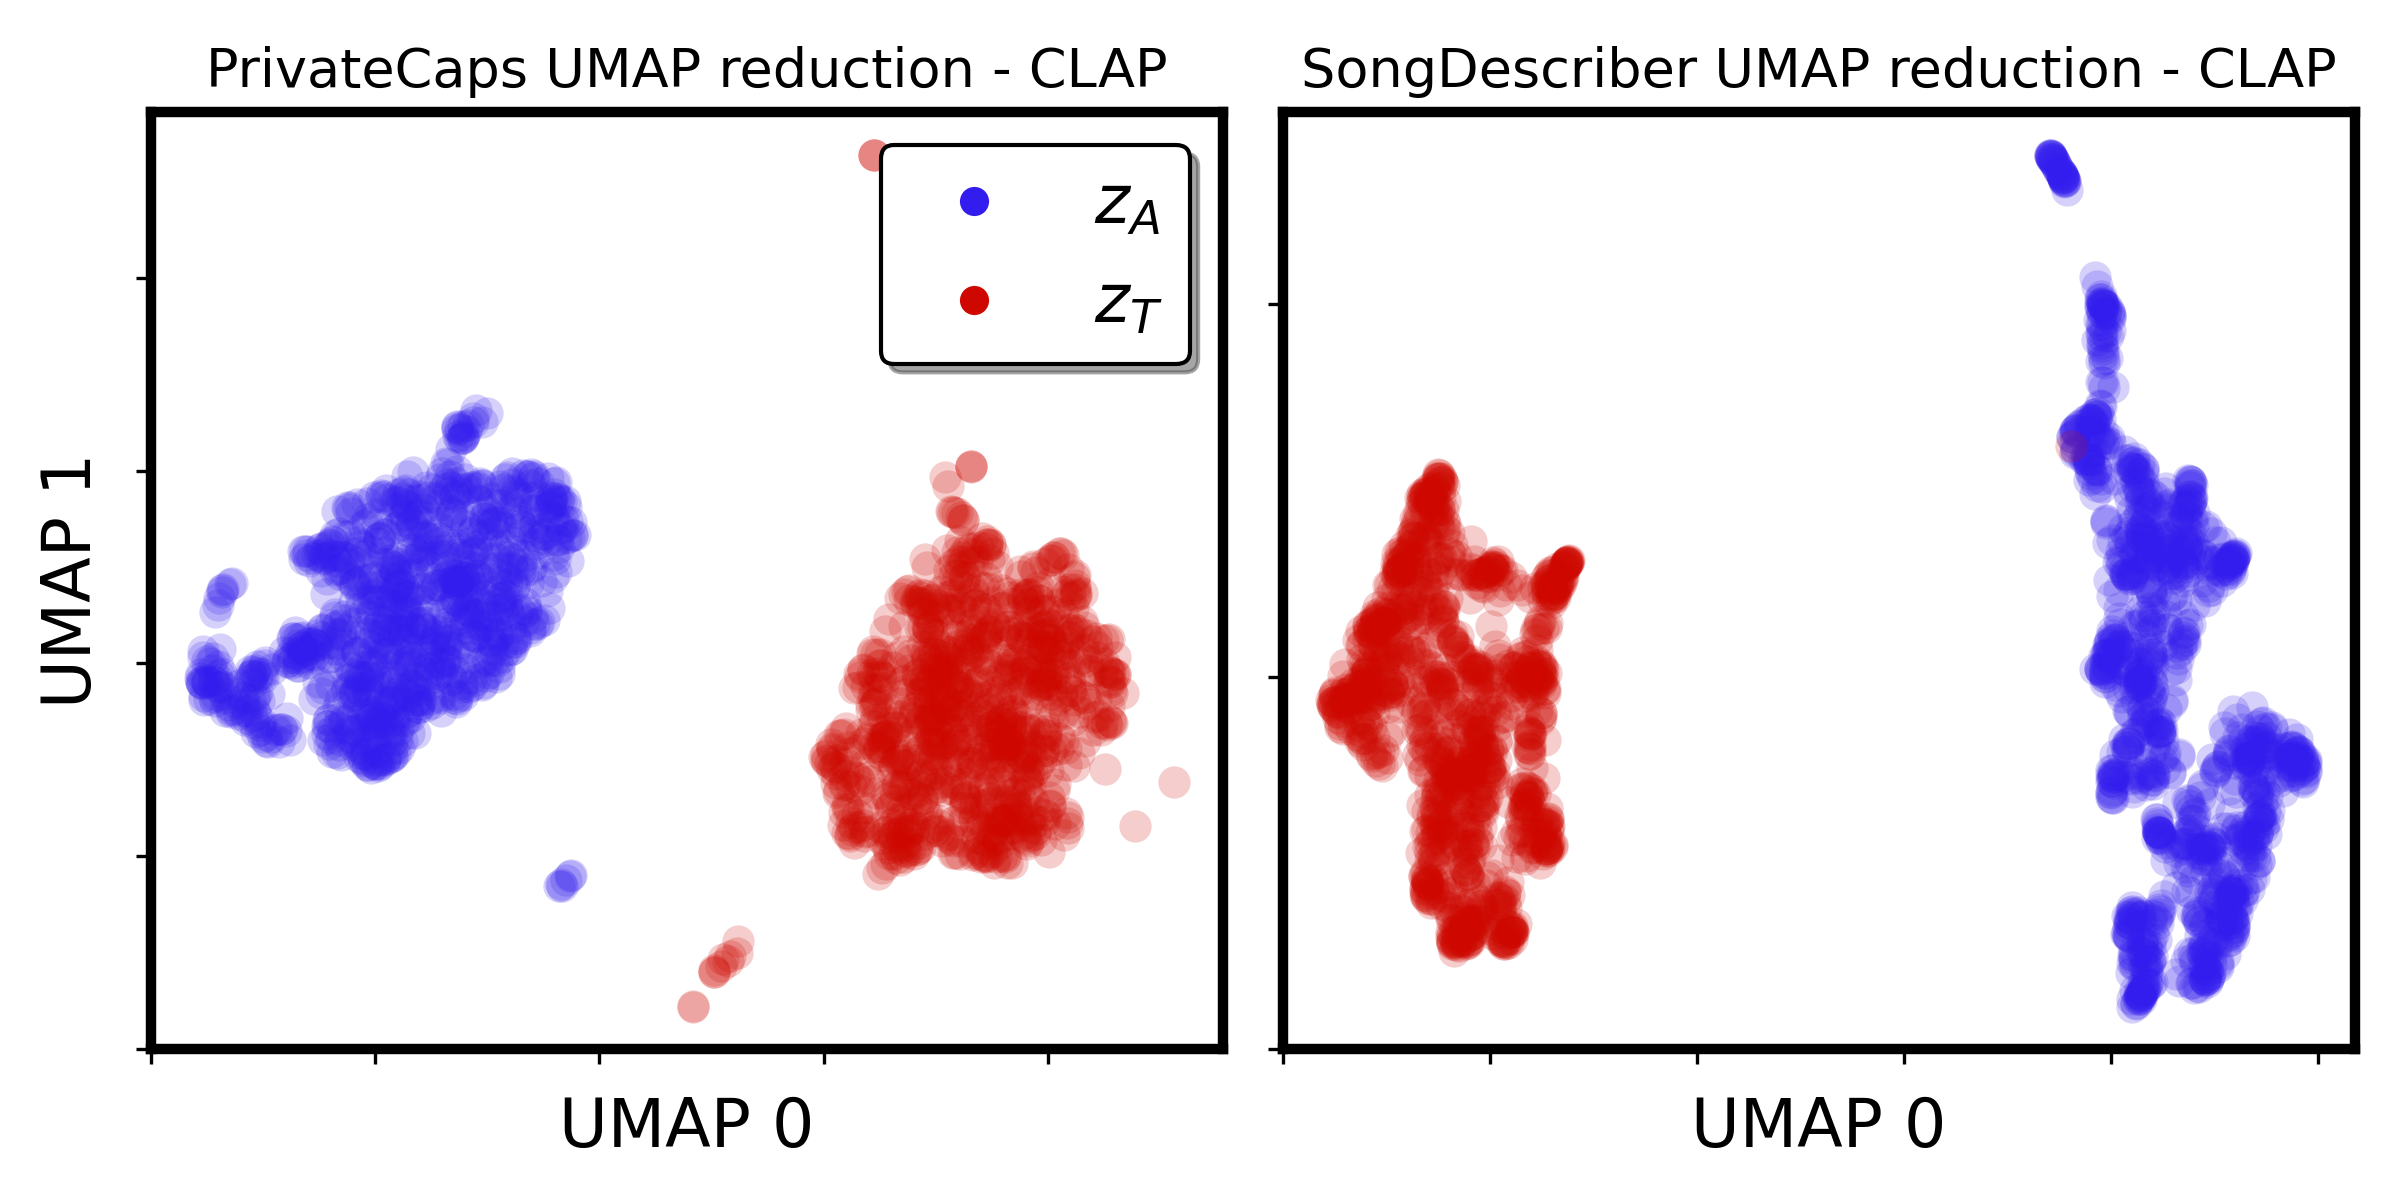
\includegraphics[width=\linewidth]{figs/umapclap.png}
%         \caption{SLAP $z$ and $q$ on PC \textbf{(left)} and SD \textbf{(right)}}
%         \label{fig:SLAPreduction}
%     \end{subfigure}
%     \hfill
%     \begin{subfigure}{1\columnwidth}
%         \centering
%         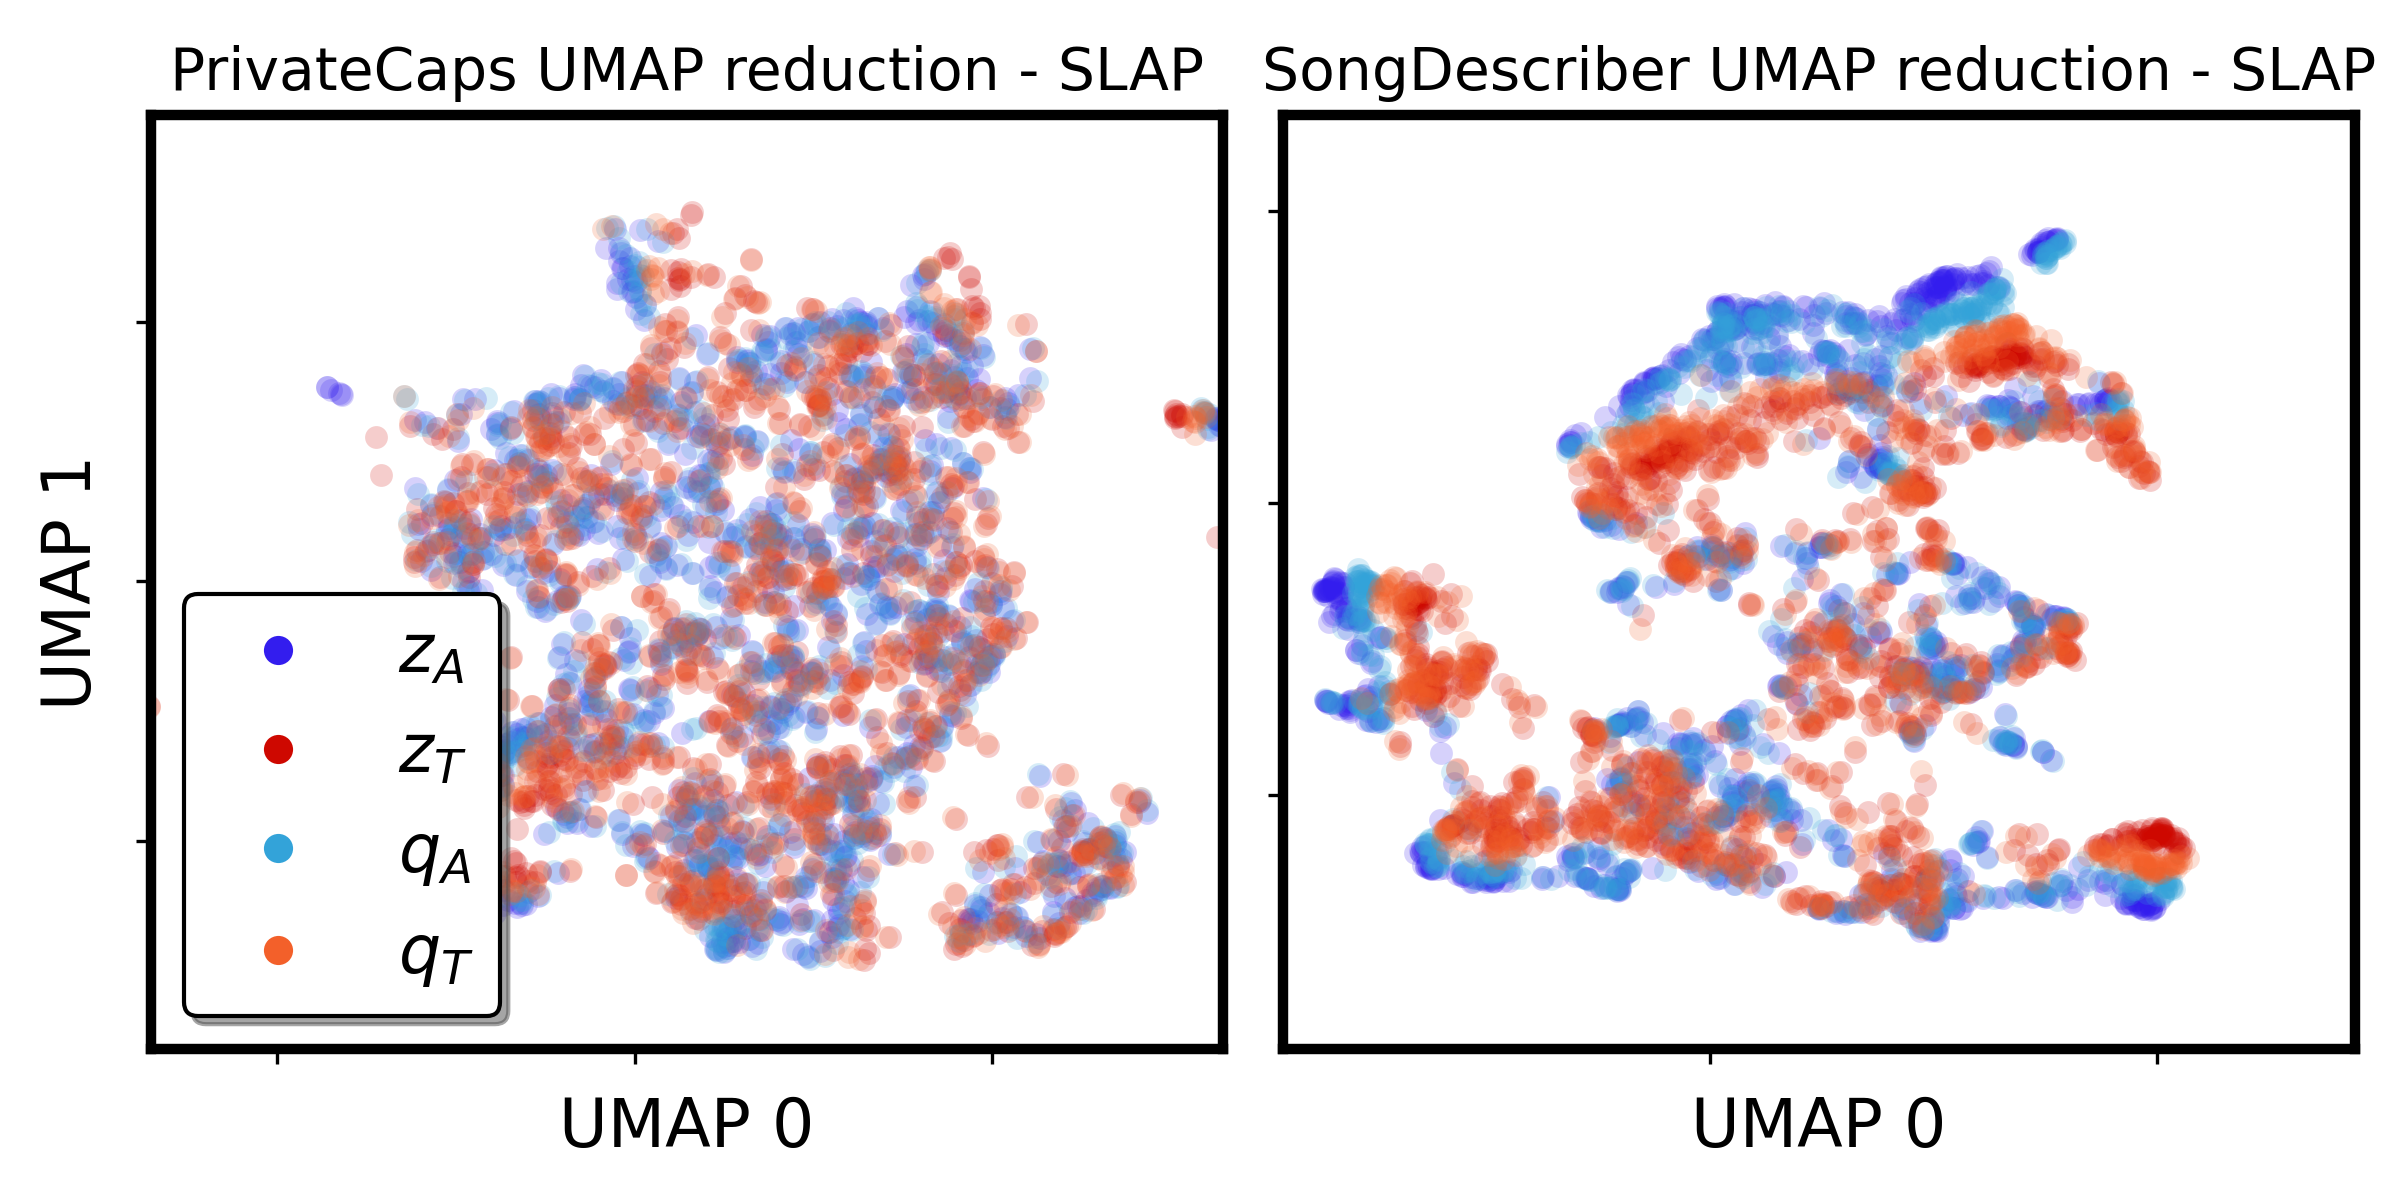
\includegraphics[width=\linewidth]{figs/umapslap.png}
%         \caption{CLAP $z$ on PC \textbf{(left)} and SD (\textbf{right})}
%         \label{fig:CLAPreduction}
%     \end{subfigure}
%     \caption{
%         UMAP Reduction of PrivateCaps (PC) and Song Describer (SD) for CLAP (\textbf{top)} and SLAP \textbf{(bottom)}.
%     }
%     \label{fig:UMAPreductions}
% \end{figure}

\begin{figure}
    % \hspace{-\columnwidth}
    \includegraphics[width=0.95\columnwidth]{figs/modalitygap.pdf}
    \caption{Centroid Distance (\textbf{left}) and Linear separability (\textbf{right}) for SLAP and CLAP on PrivateCaps, SongDescriber and MusicCaps test sets. Lower is better.}
    \label{fig:modalitygap}
\end{figure}


\subsection{Modality gap}\label{modalitygap}

As discussed in Section \ref{sec:limits}, one notable issue with MCL is the presence of a modality gap~\cite{liang2022mind,Fahim2024}.
%Early studies attribute this gap to the initialization of two different encoders for two different modalities with different architectures leading to optimal distributions of embeddings lying on different manifolds of the hypershpere \cite{liang2022mind}. However, newer interpretations show that this is not necessarily a multimodal issue, rather a direct consequence of the contrastive formulation \cite{fahim2024its}.
While it is unclear how detrimental the modality gap is to performance for retrieval, it has been shown that ``closing the gap'' is beneficial at least for generative applications \cite{nistal2024improving}.
Intuitively, having disjoint manifolds of audio and text representations allows their usage for cosine-similarity Max Inner Product Search, but is not beneficial for a shared joint understanding of text and audio. Multimodal contrastive models are subject to a modality gap, likely attributable to the non-uniformity of the latent space \cite{Fahim2024}. Not being contrastive, we posit our method should be less prone to creating a modality gap. Figure \ref{fig:UMAPreductions} shows the UMAP reduction of projections $z_T,z_A$ and $q_T,q_A$ on the test set of PrivateCaps and SD, for both CLAP and SLAP. While the modality gap of CLAP is immediately apparent, SLAP does not seem to produce an evident modality gap. and find that SLAP exhibits a strongly mitigated modality gap compared to CLAP, across datasets and training scales. 

Further, as in \cite{Fahim2024} and \cite{liang2022mind}, we report the linear separability of modalities in the latent space. typically, the modality gap manifests via different modalities existing within different manifolds of the latent spaces. If the modality gap exists, these manifolds are linearly separable, and \textit{vice-versa}. We measure linear Logistic Regression binary classification accuracy of modalities $L_{A/T}$ by overfitting a logistic regression classifier to predict the modality of embeddings on the training set. We further measure the pairwise Euclidean distance between centroids of modality embedding, i.e. the modality gap $\Delta_{A/T}$. We run this evaluation on the test sets of PrivateCaps, MusicCaps and SongDescriber (Figure \ref{fig:modalitygap}).
These findings confirm the modality gap is larger, both in terms of distance and linear separability, for CLAP than for SLAP. More so, it is nearly nonexistent for SLAP on both PC and SD. While the gap is larger for MC than for PC and SD, this can be attributed to a domain shift between datasets, likely attributable to the noisiness and longer captions of MC.

% % Please add the following required packages to your document preamble:
% % \usepackage{graphicx}
% \begin{table}[]
% \resizebox{\columnwidth}{!}{%
% \begin{tabular}{llllllllll}
% \hline
%           &  & \multicolumn{2}{c}{Audio}             & \multicolumn{2}{c}{Music}                      & \multicolumn{2}{c}{Audio}             & \multicolumn{2}{c}{Music}                      \\ \cline{3-10} 
%           &  & \multicolumn{1}{c}{AudioSet} & Clotho & \multicolumn{1}{c}{Song Describer} & MusicCaps & \multicolumn{1}{c}{AudioSet} & Clotho & \multicolumn{1}{c}{Song Describer} & MusicCaps \\ \hline
% Model     &  & \multicolumn{4}{c}{$\Delta_{A/T} \downarrow$}                                          & \multicolumn{4}{c}{$L_{A/T} \downarrow$}                                               \\ \cline{1-1} \cline{3-10} 
% AudioSLAP &  &                              &        &                                    &           &                              &        &                                    &           \\
% AudioCLAP &  &                              &        &                                    &           &                              &        &                                    &           \\ \cline{1-1} \cline{3-10} 
% MusicSLAP &  &                              &        &                                    &           &                              &        &                                    &           \\
% MusicCLAP &  &                              &        &                                    &           &                              &        &                                    &           \\ \hline
% \end{tabular}%
% }
% \caption{Modality Gap evaluation}
% \label{tab:modalitygap}
% \end{table}


\subsection{Scalability properties}



% We compare the scalability properties of SLAP versus CLAP, notably with regards to batch size. One key limitation of contrastively trained models is the loss formulation, which due to the necessity of comparing all negatives within a batch, is limited in scale. Notably, gradient accumulation does not translate to theoretically artificially increasing batch size with contrastive learning because the gradient is not linear w.r.t batch size. Theoretically, our approach does not require negatives to compute the loss, and so is ``infinitely scalable''. We also use this opportunity to study the effect of batch size on our models' performance compared to CLAP. We report $A\rightarrow$ and $T\rightarrow A$ R@1 on PrivateCaps, for CLAP and SLAP for batch sizes between 64 and 2048 used during pretraining. Batch sizes are plainly scaled for CLAP. For SLAP, the scale the base batch size of 128 by accumulating the gradient over $N$ steps to reach target batch size $B$ on a single GPU ($N = B//128$). Empirically, we verify that scaling SLAP batch size through gradient accumulation produces the same results as simply increasing the batch size. Results are reported Figure \ref{fig:Batch size scaling}.

We compare the scalability of SLAP and CLAP, focusing on batch size. A key limitation of contrastive models like CLAP is that their loss depends on all negatives in a batch, making gradient accumulation ineffective—since the gradient does not scale linearly with batch size. In contrast, SLAP requires no negatives and can theoretically be scaled to vastly large batch sizes, notably due to the lesser memory footprint and the availability of gradient accumulation. We study the effect of batch size on retrieval performance by reporting $A\rightarrow T$ and $T\rightarrow A$ R@1 on PrivateCaps for batch sizes from 64 to 768. For CLAP, batch size is scaled directly. For SLAP, we fix a base batch of 128 and accumulate gradients over $N = B // 128$ steps to reach target batch size $B$. We empirically confirm that gradient accumulation in SLAP is equivalent to true batch scaling. Results are shown in Figure~\ref{fig:Batch size scaling}.

% \vspace{-2pt}



\begin{figure}%[h]
    \centering
    \includegraphics[width=.72\columnwidth]{figs/batch_size.pdf}
    \caption{Scaling batch size for CLAP and SLAP}
    \label{fig:Batch size scaling}
\end{figure}

\subsection{Role of Intermodal and Intramodal Loss terms}\label{subsection: role of intermodal and intramodal loss terms}

One key component of our approach is the multiple loss terms between the different EMA encoders of the training setup. We find that empirically, the absence of these losses $\mathcal{L}_A$ and $\mathcal{L}_T$ leads to collapse of the model.
%as we show by reporting retrieval Recall and NMedR as well as linear separability of the modality gap
We show this in Figure \ref{fig:intermodality loss} by reporting recall@$k$ and linear separability between modalities
for different balancing weights $\lambda$.% in Figure \ref{fig:intermodality loss}.


\begin{figure}[h]
    \centering
    \includegraphics[width=1\columnwidth]{figs/ssl_weight_analysis.pdf}
    \caption{Tuning of intramodality loss balancing weight $\lambda$ for the SLAP objective, measuring both $T\rightarrow A$ and $A\rightarrow T$ retrieval performance and $L_{A/T}$.}
    \label{fig:intermodality loss}
\end{figure}

We find that within a range of $\lambda$, SLAP is robust for retrieval. Values of $\lambda$ outside [0.2, 0.7] lead to almost systematic collapse due to the lack of meaningful constraints between modalities. Despite good retrieval robustness, we find that any $\lambda \neq 0.5$ yields a rapidly increasing modality gap. Only a balanced contribution of intra and inter-modality loss terms leads to the significant reduction of the modality gap observed in Section \ref{modalitygap}.

% \subsubsection{Ablation: Variation of EMA rate and schedule}

% Our Approach is relatively robust to ema rate $\tau$, but still benefits from a rate within a certain range. In this section we explore the performance of our approach with different ema rates within the range of [0.8, 0.999] and report retrieval performance. We also briefly study the influence of EMA scheduling with three schedules: Linear, cosine annealing, and exponential with as starting point the best rate found through the previous search and as final rate $\tau=1$ over the course of training Results are reported Table \ref{}:



% \subsubsection{Ablation : Predictor hyperparameters and projection scale}

% In this section we study the influence of the scale of the predictor as well as the projection embedding dimension. By default, our predictor has a single ReLu-actived 4096-dimension layer. We train SLAP for 20 epochs with single hidden layers within the width range [512,1024,2048,4096,8192], and double layers with the same widths. Searches over predictor hyperparameters are performed with $d=512$. We also study the influence of the projector embedding dimension on Retrieval performance, with $d \in [64,128,256,512,1024]$ with the default single-layer 4096-wide MLP. Results are reported Figures \ref{fig:predictorarchitecture} and \ref{fig:embeddingscale}.

% \begin{figure}[ht]
%     \centering
%     \begin{subfigure}[b]{0.48\columnwidth}
%         \centering
%         \includegraphics[width=\linewidth]{Predictor_architecture.png}
%         \caption{Influence of predictor architecture on Retrieval performance}
%         \label{fig:predictorarchitecture}
%     \end{subfigure}
%     \hfill
%     \begin{subfigure}[b]{0.48\columnwidth}
%         \centering
%         \includegraphics[width=\linewidth]{Embedding_scale.png}
%         \caption{Influence of embedding dimension $d$ on Retrieval performance}
%         \label{fig:embeddingscale}
%     \end{subfigure}
%     \caption{Retrieval performance evolution with varying predictor architectures and different project embedding scales.}
%     \label{fig:overall_figure}
% \end{figure}

% \subsubsection{Ablation : Normalisation of prediction and projection}

% In the original BYOL \cite{grill2020bootstrap}, normalisation of the predictor outputs has a non-negligible influence on performance. We also aim to understand the influence of normalisation on the performance of SLAP. While we always leave l2-normalization applied to predictions and projections for the losses, we explore applying optional batch normalization to the outputs of the projection head and predictors through 1D-BatchNorm layers. Changes in retrieval results are reported Table \ref{}.

\section{Conclusion and future work}

% In this work, we propose a novel approach to training multimodal joint embedding spaces applied to music and text, Siamese Language Audio Pretraining. Through training our model on a medium-scale dataset of high-quality text-music caption pairs, we outperform comparable contrastively-trained models on a range of tasks, including text-music retrieval downstream probing, and zero-shot probing on music understanding tasks. We further show desirable attributes of our approach over contrastive approaches, including negative-free training which leads to improved scalability, as well as strong mitigation of the modality gap that arises from contrastive training. Without implementing any extensive text, audio augmentation strategies, further architectural improvements aiming to improve contrastive training, nor heavy hyperparameter optimization, we approach state of the art performance on many of these tasks, showing the promise of SLAP as a replacement for CLAP approaches. While remaining free of any complex machinery, SLAP promotes a scalable approach to multimodal representation learning which can be directly applied to more than two modalities.\\

We propose a novel approach to training multimodal joint embedding spaces to align music and text representation: Siamese Language Audio Pretraining (SLAP). SLAP outperforms contrastive models on tasks including text-music retrieval, downstream probing, and zero-shot music understanding. It offers key advantages over contrastive approaches, including negative-free training for better scalability and substantial reduction of the modality gap. Without relying on extensive data augmentation, architectural tuning, or hyperparameter optimization, SLAP matches state-of-the-art performance—demonstrating its potential as a scalable alternative to CLAP-style training.

Several works have built upon CLIP/CLAP to improve its downstream performances, e.g., by exploring alternative architectures~\cite{elizalde2023clap,CyCLAP}, scaling-up training data~\cite{ghosh2025reclap,AudioFlamingo2}, promoting semantic or linguistic invariance~\cite{MaskCLIP,AudioFlamingo2} or improving the sensitivity to fine-grained temporal events~\cite{yuan2024t,wu2024collap}.
These improvements do not exploit the contrastive loss and SLAP could probably benefit from them as well.

Finally, while we demonstrate the effectiveness of our method on music-related tasks, it is generalizable and could be applied to other modalities such as images or general audio. We therefore believe that this approach could lead to many applications beyond the scope of our paper.

%Recent work has enhanced CLIP/CLAP via architectural changes~\cite{elizalde2023clap,CyCLAP}, large-scale pretraining~\cite{ghosh2025reclap,AudioFlamingo2}, semantic robustness~\cite{MaskCLIP,AudioFlamingo2}, or improved temporal sensitivity~\cite{yuan2024t,wu2024collap}. SLAP's formulation is compatible with these techniques and could likely benefit from them as well. While our results focus on music, SLAP has the potential to be modality-agnostic, and could be extended to other domains such as image, general audio, or the combination thereof, opening promising directions for future multimodal applications.


%We did not apply the study-specific techniques proposed in follow-up work to CLAP, which aimed to reduce the modality gap or improve fine-grained understanding between timesteps and individual tokens, to compare core methodologies between contrastive and siamese training. However, the loss modification of SLAP is not prohibitive to any of these techniques, nor is its stability over hyperparameters. Hence, SLAP is compatible with all other improvements proposed for CLAP. We encourage future work to apply these CLAP techniques to SLAP to further improve performance. Future work should additionally focus on further exploring the design space of SLAP to understand the best combination of hyperparameters such as predictor scale, EMA schedule, and embedding scale for optimal performance.
%Improving joint text-audio embedding spaces is a vibrant research area, and current prevalent research directions include improving fine-grained understanding between individual text tokens and audio segments \cite{}, and enhancing caption augmentation strategies to increase the scale of training data \cite{}. The former aims to mitigate lossy information compression due to pooling in contrastive learning. Inspired by text-image representation learning \cite{}, recent work has focused on early fusion of modality information \cite{} or informed pooling before applying the contrastive objective \cite{}. The latter addresses the scarcity of public audio-text pair training data compared to image-text pairs by employing large language model (LLM) augmentation for captions \cite{} or mining improved negatives and positives for existing captions \cite{}. While both approaches have shown notable improvements in joint-embedding text-audio representation performances, neither addresses the core training paradigm of contrastive learning itself.

\comm{
\begin{itemize}
    % \item pdf plutôt que png pour les figures
    % \item le truc du mAR c pas convaincant
    % \item linear separability c pas censé être entre 0.5 et 1?
    \item la baseline de la table 2 c pas clair ce que c'est et ce que ça fout là
    \item ethical statement? les data sont clean, on publie le code mais pas les data, est-ce qu'on en parle? + applications en génératif? licence sur le code pour prevent les malicious usages?
    \item si on a trop de place autant faire une conclusion plus sexy:
    - CLIP / SigLIP / CLAP c des powerful encoders et tous les multimodal LLM utilisent ça as a backbone donc être meilleur que CLAP ça veut dire des meilleurs multimodal LLM
    - résoudre le modality gap ça permet d'être meilleur sur tous les trucs de multimodal conditioning
    - 5.4 les abbréviations c'est pas consistent + les metrics de la figure c'est bien sur les queries?
\end{itemize}}

\clearpage

\bibliography{refs}

% \input{tables/autoacd}

% %% MAIN RESULTS
% CLAP vs SLAP trained on AutoACD (Recall $(\uparrow)$, MR) - Not focused on music
% CLAP VS SLAP trained on UMG (Recall $(\uparrow)$, NR) - Music focused
% projection retrieve projection vs prediction retrieve prediction

% % Linear downstream tasks
% embeddings, projections, predictions

% % modality gap
% - classifier-based (predicting modality) % 
% - classifier on predictions vs projections
% https://arxiv.org/pdf/2405.18570
% - mesurer la distance entre les centroids
% - petits plots

% %% Zero-shot 

% %% ablations
% - batch size
% - better encoders (RoBERTa vs betterBERT, ViT vs HTSaT)
% - normalization


\end{document}




% pretrained either vs both
∞ length of captions bottleneck for performance